\documentclass{beamer}[10]

\usepackage{graphicx}
\usepackage{xcolor}
\usepackage{tabto}
%\usepackage{beamerthemesplit}
\usepackage{tikz}
\usepackage{cancel}
\usepackage{verbatim}
\usepackage{fancybox}
\usepackage{enumerate}
\usepackage{amsmath,amssymb,amsthm,textcomp,mathtools}
\usepackage[super]{nth}
\usepackage[amssymb]{SIunits}
\usepackage{booktabs}
\usepackage{cancel}
\usepackage{bm}
\usepackage[utf8]{inputenc}
\usepackage{tabularx}
\usepackage{ragged2e}
\newcolumntype{Y}{ >{\RaggedRight\arraybackslash}X}
\usetikzlibrary{arrows,shapes}
\newcommand\T{\rule{0pt}{2.6ex}}
\newcommand\B{\rule[-1.2ex]{0pt}{0pt}}
\definecolor{UUcrimson}{RGB}{204,0,0}
\mode<presentation>
{ \usetheme{default}
  \usecolortheme[named=UUcrimson]{structure}
  \useinnertheme{circles}
  \setbeamercovered{transparent}
  \setbeamertemplate{blocks}[rounded]
  \usefonttheme[onlymath]{serif}
  \setbeamertemplate{navigation symbols}{}
  \setbeamertemplate{footline}[page number]
  \setbeamertemplate{navigation symbols}{}
  \setbeamercolor{section in toc}{fg=black,bg=white}
  \setbeamercolor{alerted text}{fg=UUcrimson!80!gray}
  \setbeamercolor*{palette primary}{fg=white,bg=UUcrimson}
  \setbeamercolor*{palette secondary}{fg=UUcrimson!70!black,bg=gray!15!white}
  \setbeamercolor*{palette tertiary}{bg=UUcrimson!80!black,fg=gray!10!white}
  \setbeamercolor*{palette quaternary}{fg=UUcrimson,bg=gray!5!white}
  \setbeamercolor*{palette sidebar primary}{fg=UUcrimson!10!black}
  \setbeamercolor*{palette sidebar secondary}{fg=white}
  \setbeamercolor*{palette sidebar tertiary}{fg=UUcrimson!50!black}
  \setbeamercolor*{palette sidebar quaternary}{fg=gray!10!white}
  \setbeamercolor{titlelike}{parent=palette primary,fg=white}
  \setbeamercolor{frametitle}{bg=UUcrimson}
  \setbeamercolor{frametitle right}{bg=UUcrimson}
  \setbeamercolor*{separation line}{}
  \setbeamercolor*{fine separation line}{}
}

\usetikzlibrary{backgrounds}
\makeatletter
\tikzstyle{every picture}+=[remember picture]
\tikzset{%
  fancy quotes/.style={
    text width=\fq@width pt,
    align=justify,
    inner sep=1em,
    anchor=north west,
    minimum width=\linewidth,
    font=\itshape
  },
  fancy quotes width/.initial={.8\linewidth},
  fancy quotes marks/.style={
    scale=8,
    text=white,
    inner sep=0pt,
  },
  fancy quotes opening/.style={
    fancy quotes marks,
  },
  fancy quotes closing/.style={
    fancy quotes marks,
  },
  fancy quotes background/.style={
    show background rectangle,
    inner frame xsep=0pt,
    background rectangle/.style={
      fill=gray!25,
      rounded corners,
    },
  }
}
\newenvironment{fancyquotes}[1][]{%
\noindent
\tikzpicture[fancy quotes background]
\node[fancy quotes opening,anchor=north west] (fq@ul) at (0,0) {``};
\tikz@scan@one@point\pgfutil@firstofone(fq@ul.east)
\pgfmathsetmacro{\fq@width}{\linewidth - 2*\pgf@x}
\node[fancy quotes,#1] (fq@txt) at (fq@ul.north west) \bgroup}
{\egroup;
\node[overlay,fancy quotes closing,anchor=east] at (fq@txt.south east) {''};
\endtikzpicture}
\makeatother


\usetikzlibrary{backgrounds}
\makeatletter
\tikzstyle{every picture}+=[remember picture]
\tikzset{%
  fancy defs/.style={
    text width=\fq@width pt,
    align=justify,
    inner sep=0.25em,
    anchor=north west,
    minimum width=\linewidth,
    font=\itshape
  },
  fancy defs width/.initial={.8\linewidth},
  fancy defs marks/.style={
    scale=8,
    text=white,
    inner sep=0pt,
  },
  fancy defs opening/.style={
    fancy defs marks,
  },
  fancy defs closing/.style={
    fancy defs marks,
  },
  fancy defs background/.style={
    show background rectangle,
    inner frame xsep=0pt,
    background rectangle/.style={
      fill=gray!25,
      rounded corners,
    },
  }
}
\newenvironment{fancydefs}[1][]{%
\noindent
\tikzpicture[fancy defs background]
\node[fancy defs opening,anchor=north west] (fq@ul) at (0,0) {};
\tikz@scan@one@point\pgfutil@firstofone(fq@ul.east)
\pgfmathsetmacro{\fq@width}{\linewidth - 2*\pgf@x}
\node[fancy defs,#1] (fq@txt) at (fq@ul.north west) \bgroup}
{\egroup;
\node[overlay,fancy defs closing,anchor=east] at (fq@txt.south east) {};
\endtikzpicture}
\makeatother
\usepackage{scalerel}[2014/03/10]
\usepackage{stackengine}
\usepackage{empheq}
\newcommand*\widefbox[1]{\fbox{\hspace{0.5em}#1\hspace{0.5em}}}

\newcommand\reallywidetilde[1]{\ThisStyle{%
  \setbox0=\hbox{$\SavedStyle#1$}%
  \stackengine{-.1\LMpt}{$\SavedStyle#1$}{%
    \stretchto{\scaleto{\SavedStyle\mkern.2mu\sim}{.5467\wd0}}{.4\ht0}%
%    .2mu is the kern imbalance when clipping white space
%    .5467++++ is \ht/[kerned \wd] aspect ratio for \sim glyph
  }{O}{c}{F}{T}{S}%
}}
\usepackage{media9}

\logo{
\includegraphics[width=0.75cm]{logo.jpg}}
\author[Gibbs]{Dr. Jeremy A. Gibbs}
\institute{Department of Mechanical Engineering\\University of Utah}
\date{Spring 2017}
\title{Environmental Fluid Dynamics: Lecture 3}
% colors
\definecolor{colororange}{HTML}{E65100} % orange
\definecolor{colordgray}{HTML}{795548} % dark gray for note
\definecolor{colorhgray}{HTML}{212121} % heavy dark gray for normal text
\definecolor{colorgreen}{HTML}{009688} % green
\definecolor{colorwhite}{HTML}{FFFFFF} % background white
\definecolor{colorlgray}{HTML}{F5F3EE} % background light gray
\definecolor{colorblue}{HTML}{0277BB} % blue
\definecolor{colorred}{HTML}{CC0000} % red
\newcommand{\fontsizeone}{1.9em}
\setbeamertemplate{caption}{\raggedright\insertcaption\par}
\newcommand{\framecard}[2][colorgreen]{
  {\setbeamercolor{background canvas}{bg=#1}
    \begin{frame}[plain]
    \vfill
    \begin{center}
     {#2}
    \end{center}
    \vfill
    \end{frame}
  }
}

\begin{document}

%----------------------------------------------------------------------------------------
%	TITLE & TOC SLIDES
%----------------------------------------------------------------------------------------

\begin{frame} 
  \titlepage
\end{frame}

%------------------------------------------------

\begin{frame}
\frametitle{Overview}
\tableofcontents
\end{frame}

%------------------------------------------------
\section{A Few More Things About Radiation} %
%------------------------------------------------
\framecard[colorred]{{\color{white}\Huge A Few More Things About Radiation}}
%------------------------------------------------
\begin{frame}{Black Body Radiation}
From Bergman et al. (2011):
\begin{fancydefs}
A black body absorbs all incident radiation, regardless of wavelength and direction
\end{fancydefs}

\begin{itemize}
	\item for a prescribed temperature and wavelength, no surface can emit more energy than a blackbody
	\item Although the radiation emitted by a black body is a function of wavelength and temperature, it is independent of direction (\textit{i.e.}, the blackbody is a diffuse emitter)
	\item a blackbody is a perfect absorber and emitter, letting it serve as the standard against which the radiative properties of actual surfaces may be compared
\end{itemize}
\end{frame}

%------------------------------------------------
\begin{frame}{Black Body Radiation}
\begin{columns}[T]
    \begin{column}{.4\textwidth}
    \begin{minipage}[c][0.8\textheight][c]{\linewidth}
    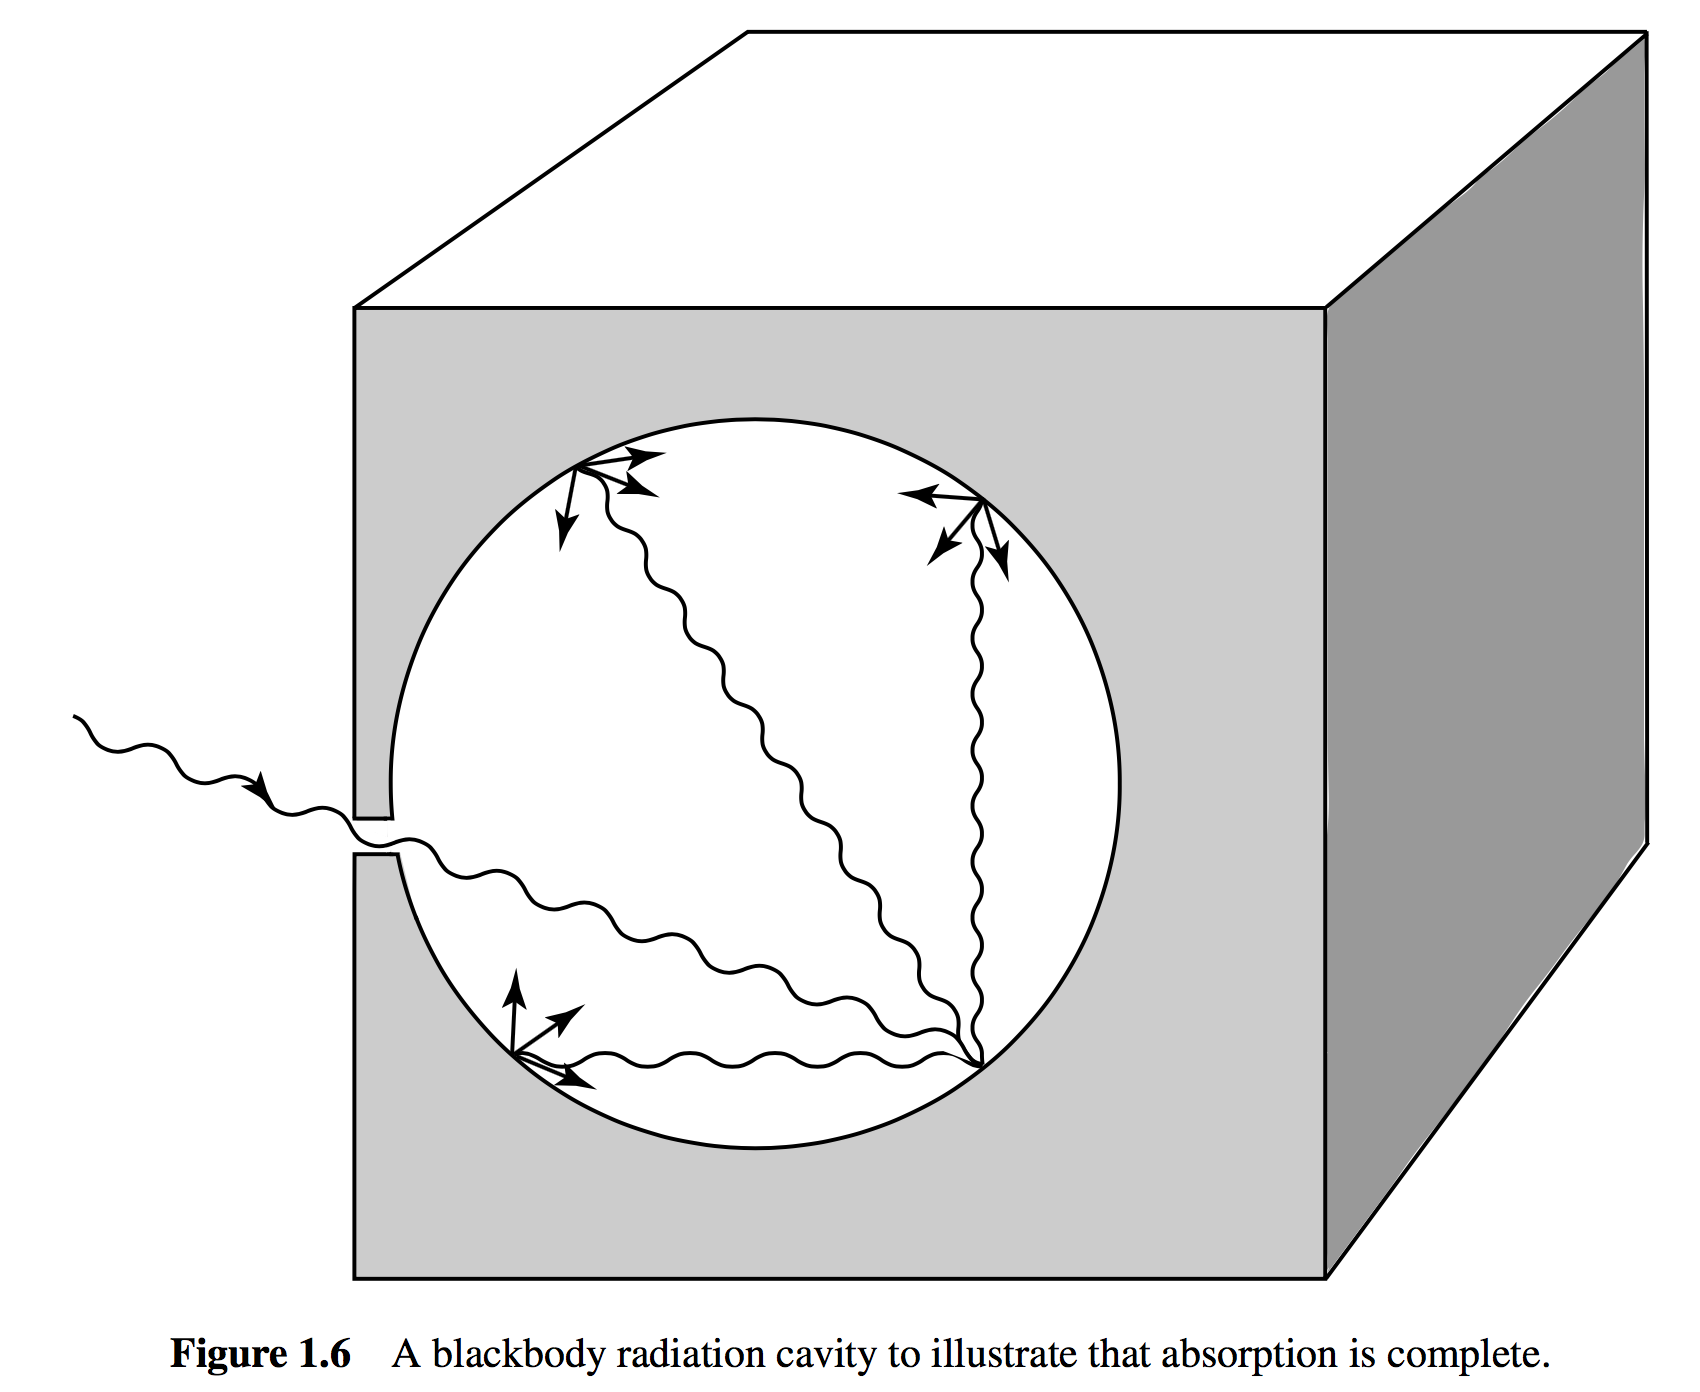
\includegraphics[width=1\textwidth]{fig13.png}\\
    \centering \small From Liou (2002)
    \end{minipage}
    \end{column}
    \begin{column}{.6\textwidth}
    \begin{minipage}[c][0.8\textheight][c]{\linewidth}
   \begin{itemize}
   	\item consider a cavity with a small entrance hole
   	\item most radiant flux entering this hole will be trapped within the cavity
   	\item this occurs regardless of the material and surface properties of the wall
   \end{itemize}
      \end{minipage}
    \end{column}
  \end{columns} 
\end{frame}

%------------------------------------------------
\begin{frame}{Black Body Radiation}
\begin{columns}[T]
    \begin{column}{.4\textwidth}
    \begin{minipage}[c][0.8\textheight][c]{\linewidth}
    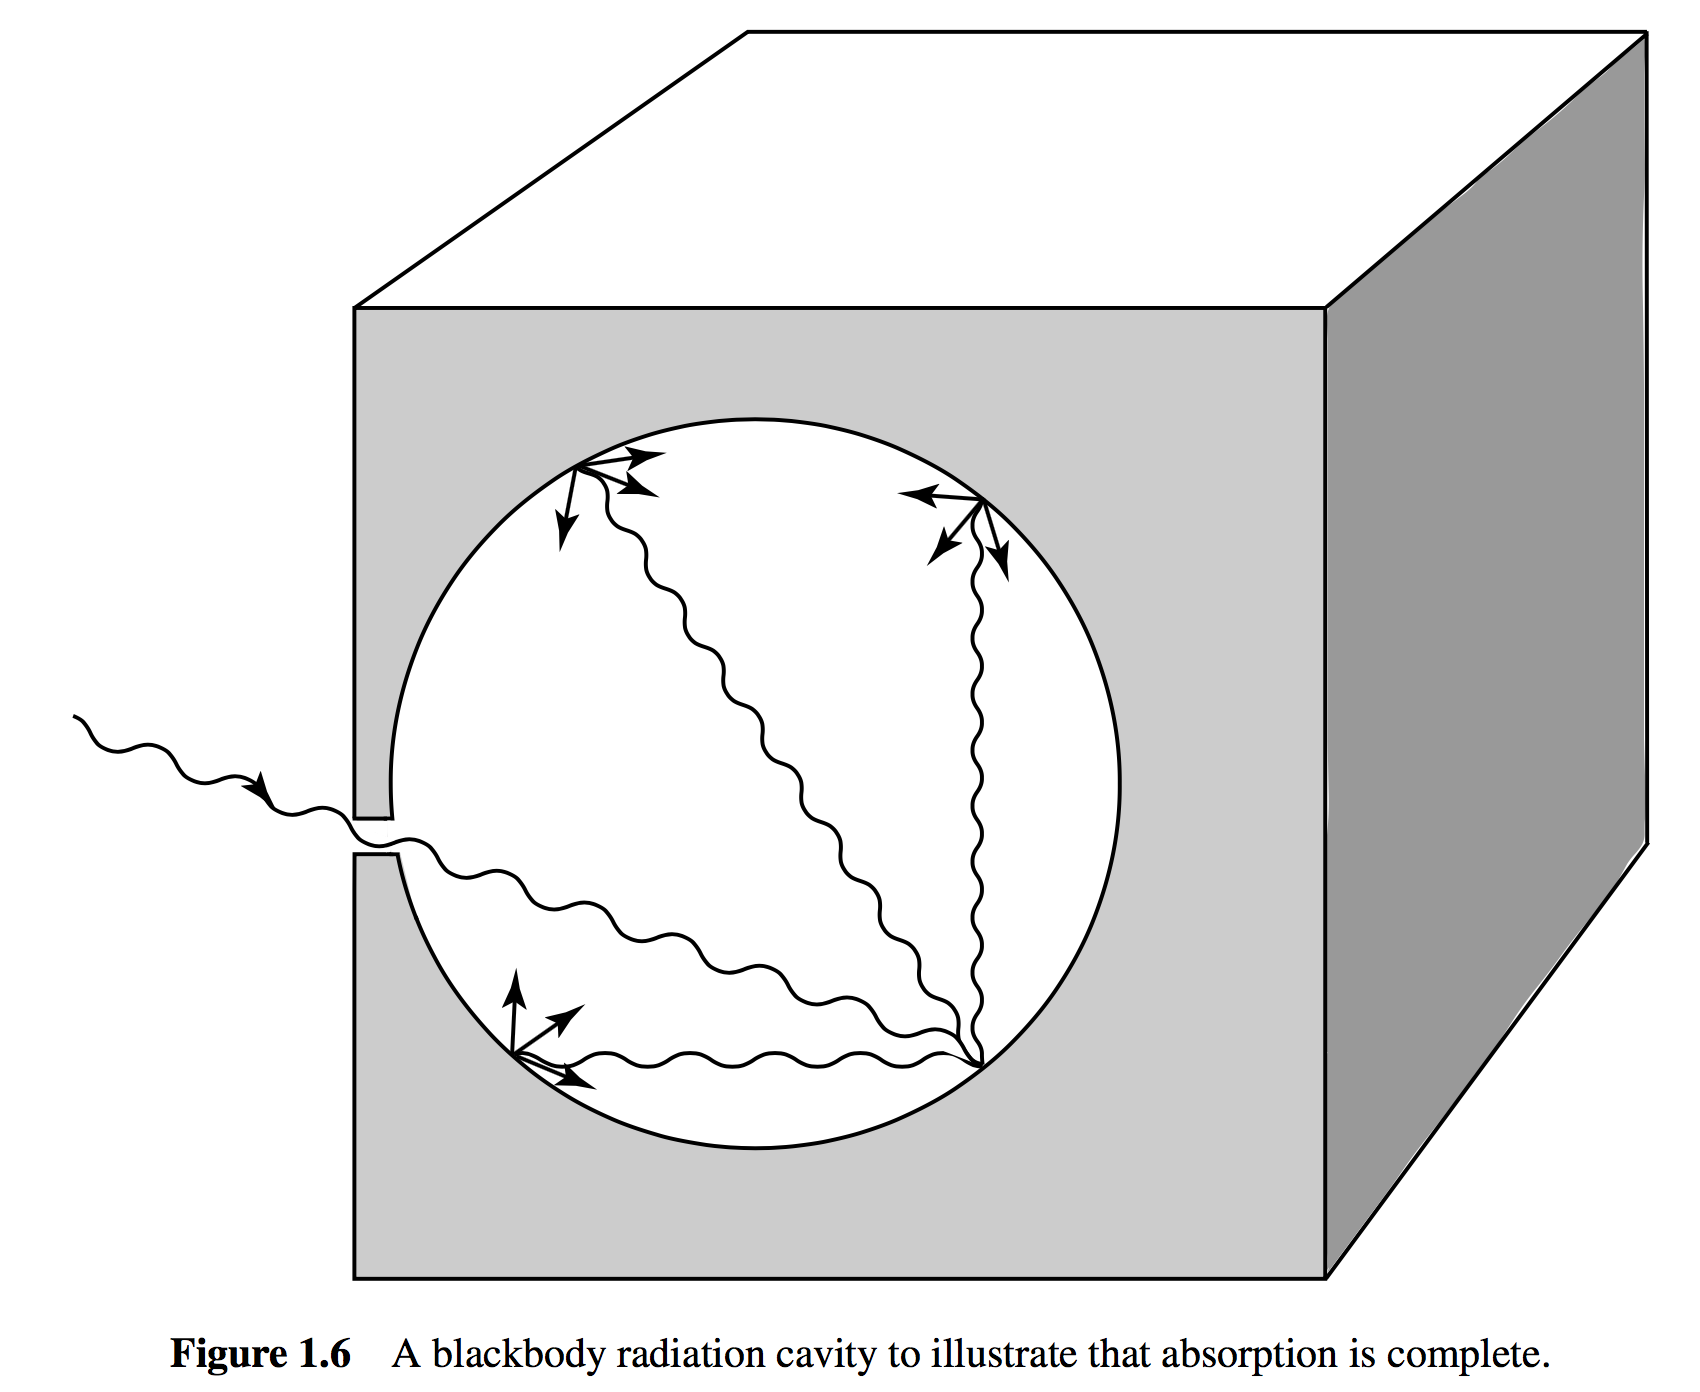
\includegraphics[width=1\textwidth]{fig13.png}\\
    \centering \small From Liou (2002)
    \end{minipage}
    \end{column}
    \begin{column}{.6\textwidth}
    \begin{minipage}[c][0.8\textheight][c]{\linewidth}
   \begin{itemize}
   	\item internal reflections occur until all the fluxes are absorbed by the wall
   	\item chance that any of the entering flux will escape back through the hole is so small that the interior appears dark
   	\item \textit{blackbody} is used for a configuration of material where absorption is complete
   \end{itemize}
      \end{minipage}
    \end{column}
  \end{columns} 
\end{frame}

%------------------------------------------------
\begin{frame}{Planck's Law}
From Bergman et al. (2011):
\begin{fancydefs}
Planck's Law describes the blackbody spectral emissive power
\begin{align*}
E_{\lambda,T} (\lambda,T) &= \frac{C_1}{\lambda^5 \left[\exp (C_2/ \lambda T) - 1 \right] }\\
\text{where}\\
C_1 &= 3.742 \times 10^8\ \watt \micro\metre^4 \metre\rpsquared\\
C_2 &= 1.439 \times 10^4\ \micro\metre\ \kelvin	
\end{align*}
\end{fancydefs}
\end{frame}

%------------------------------------------------
\begin{frame}{Planck's Law}
From Bergman et al. (2011):
\begin{fancydefs}
\begin{align*}
E_{\lambda,T} (\lambda,T) &= \frac{C_1}{\lambda^5 \left[\exp (C_2/ \lambda T) - 1 \right] }
\end{align*}
\end{fancydefs}
\begin{itemize}
	\item blackbody radiant intensity increases with temperature
	\item wavelength of the maximum intensity decreases with increasing temperature
\end{itemize}
\end{frame}

%------------------------------------------------
\begin{frame}{Planck's Law}
From last class, this is Planck's Law
\begin{figure}
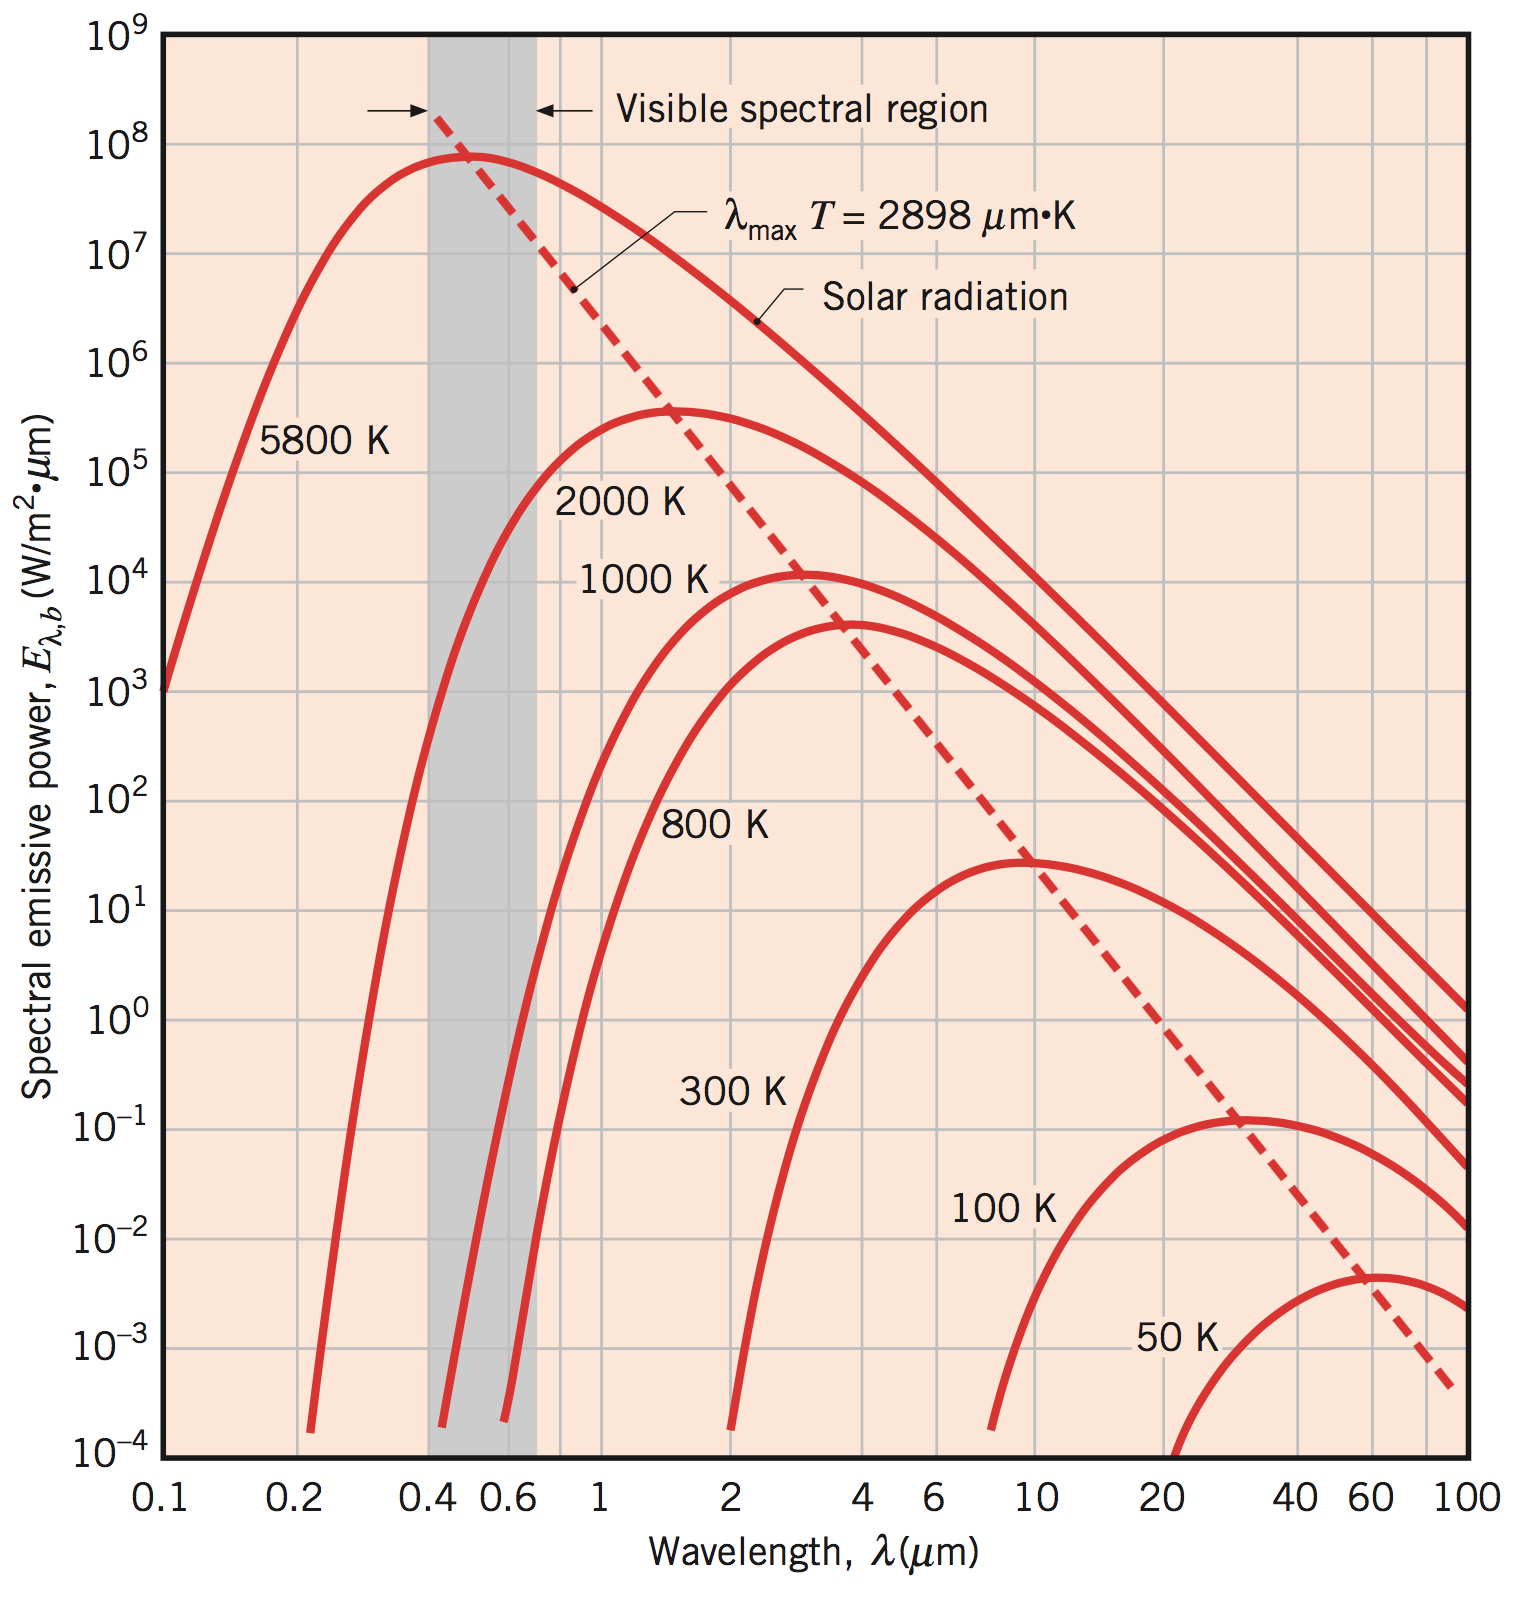
\includegraphics[width=0.65\textwidth]{fig1.png}	
\centering \tiny~\\Bergman et al. (2011)
\end{figure}
\end{frame}
%------------------------------------------------
\begin{frame}{Stefan-Boltzman Law}
\begin{itemize}
\item The total hemispherical missive power (the rate that radiation is emitted per unit area at all wavelengths and in all direction) is
$$E=\int^{\infty}_0 E_\lambda (\lambda) d\lambda$$
\item Substituting Planck's Law into this equation gives
$$E=\int^{\infty}_0 \frac{C_1}{\lambda^5 \left[\exp (C_2/ \lambda T) - 1 \right] }d\lambda$$
\item Performing the integration yields the Stefan-Boltzman Law
\end{itemize}
\end{frame}
%------------------------------------------------
\begin{frame}{Stefan-Boltzman Law}
\begin{fancydefs}
	Gives the amount of radiation emitted in all directions and over all wavelengths simply from knowledge of the temperature of the blackbody
	\begin{align*}
	E_b &= \sigma T^4\\
	\text{where}\\
	\sigma &= 5.670 \times 10^{-8}\ \watt \metre\rpsquared\ \kelvin^{-4}
	\end{align*}
\end{fancydefs}
In practice, the Law is usually written in terms of an object's emissivity $\epsilon$. For the surface of the Earth:
$$R_{L\uparrow} = -\epsilon \sigma T_s^4$$
Note: minus sign because we are talking about upward directed radiation
\end{frame}

%------------------------------------------------
\begin{frame}{Stefan-Boltzman Law}
\begin{fancydefs}
	\begin{align*}
	E_b &= \sigma T^4\\
	\text{where}\\
	\sigma &= 5.670 \times 10^8\ \watt\ \metre\rpsquared\ \kelvin^4
	\end{align*}
\end{fancydefs}
\begin{itemize}
	\item the flux density emitted by a blackbody is proportional to the \nth{4} power of the absolute temperature
	\item the S-B law is fundamental to the analysis of broadband infrared radiative transfer
\end{itemize}
\end{frame}

%------------------------------------------------
\begin{frame}{Wein's Displacement Law}
It is obtained by differentiating Planck's Law with respect to wavelength and setting the result to zero
	$$\frac{\partial E_{\lambda,T}}{\partial \lambda} = 0$$
	The results gives Wein's Displacement Law
\begin{fancydefs}
	The wavelength of the maximum intensity of blackbody radiation is inversely proportional to the temperature
	$$\lambda_m = \frac{a}{T}$$
	where $a = 2898\ \metre\ \kelvin$
	\end{fancydefs}
\end{frame}

%------------------------------------------------
\begin{frame}{Wein's Displacement Law}
\begin{fancydefs}
	The wavelength of the maximum intensity of blackbody radiation is inversely proportional to the temperature
	$$\lambda_m = \frac{a}{T}$$
	where $a = 2898\ \metre\ \kelvin$
	\end{fancydefs}
\begin{itemize}
	\item one can determine the temperature of a blackbody from the measurement of the maximum intensity
	\item this dependence of maximum intensity on temperature is clearly seen in the previous figure when discussing Planck's Law
\end{itemize}
\end{frame}

%------------------------------------------------
\begin{frame}{Wein's Displacement Law}
Note the dependence of peak intensity location on temperature
\begin{figure}
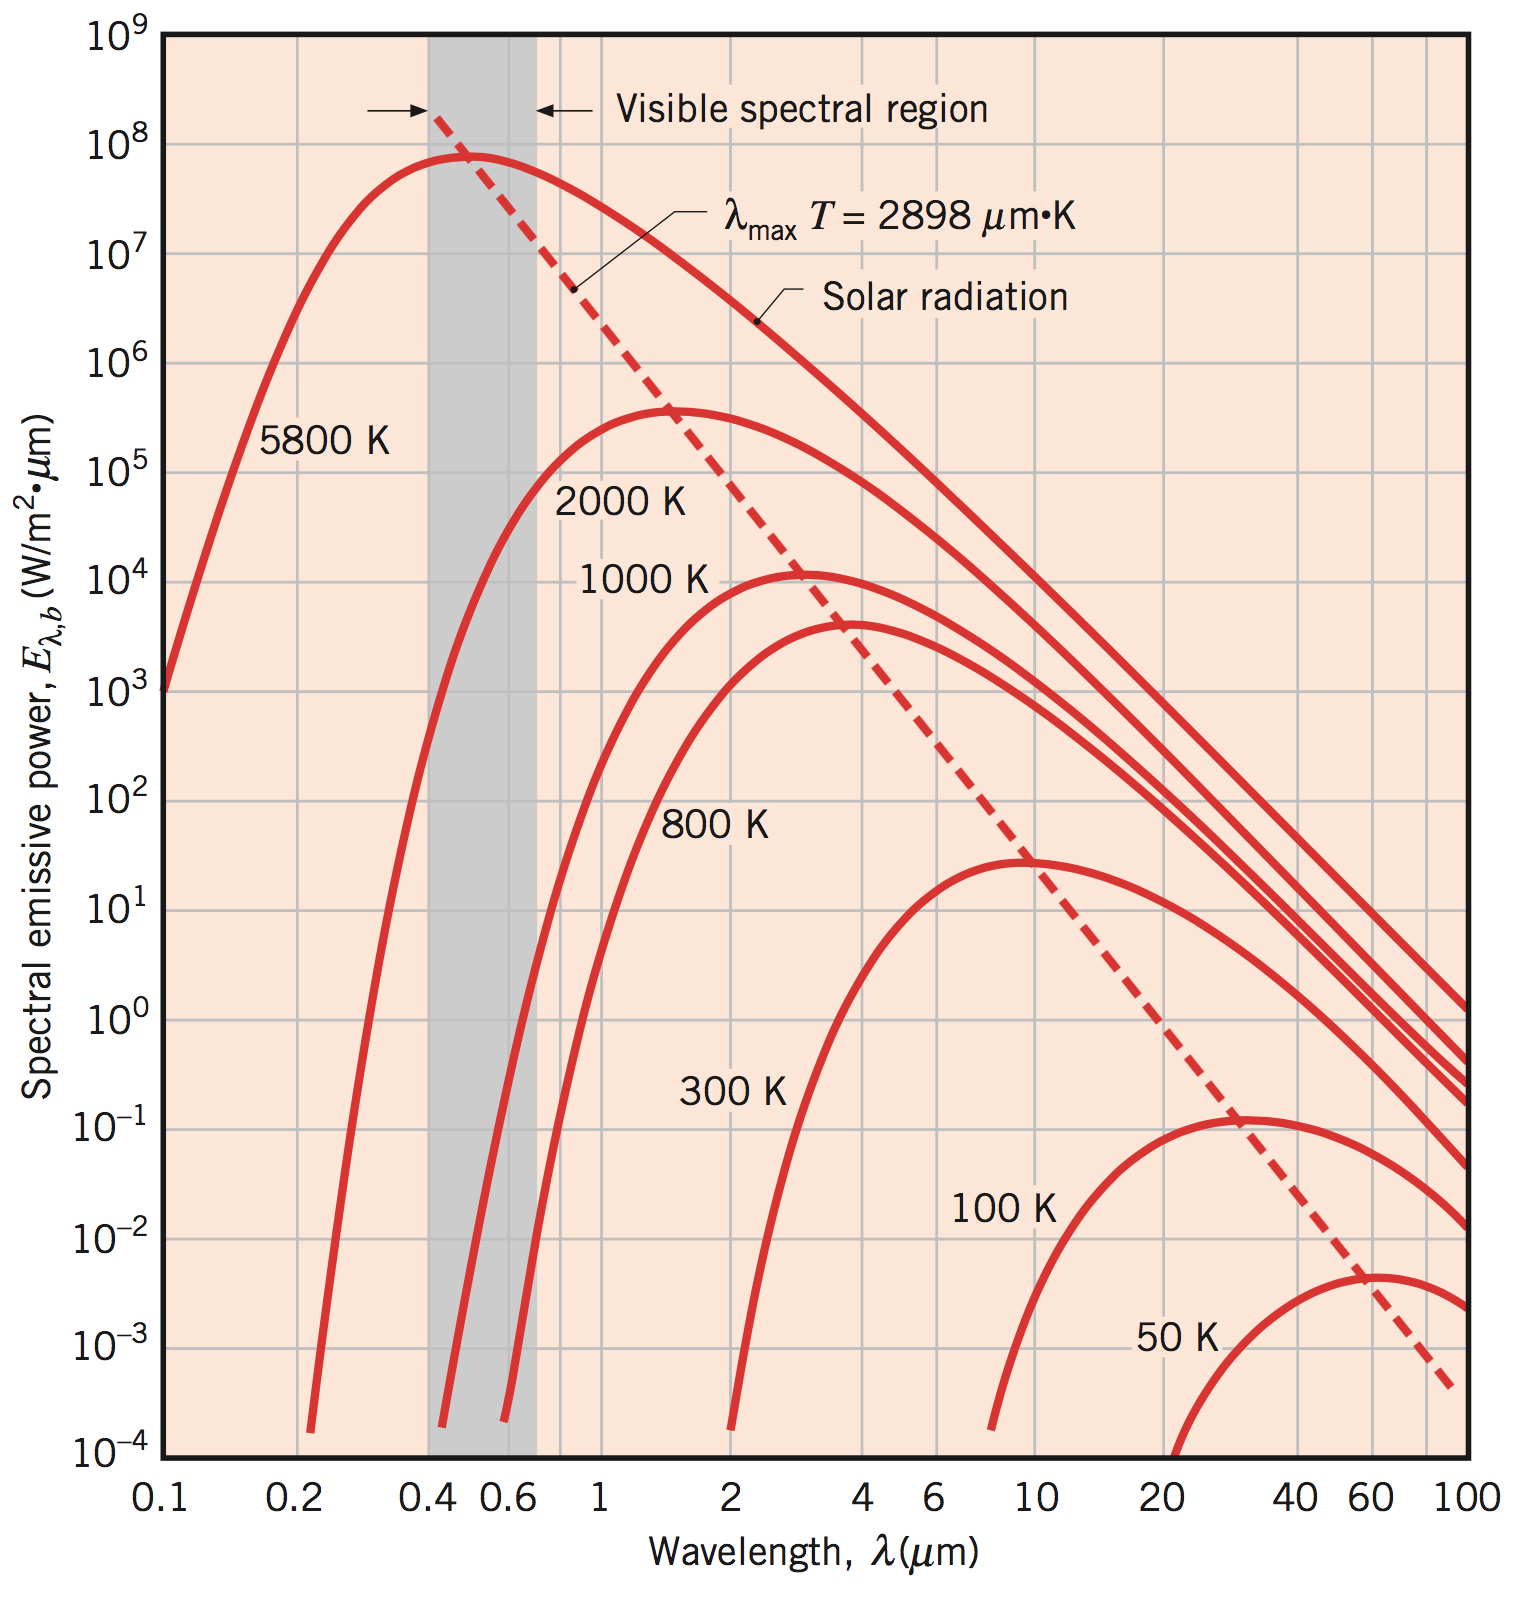
\includegraphics[width=0.65\textwidth]{fig1.png}	
\centering \tiny~\\Bergman et al. (2011)
\end{figure}
\end{frame}

%------------------------------------------------
\begin{frame}{Kirchhoff's Law}
\begin{columns}[T]
    \begin{column}{.4\textwidth}
    \begin{minipage}[c][0.8\textheight][c]{\linewidth}
    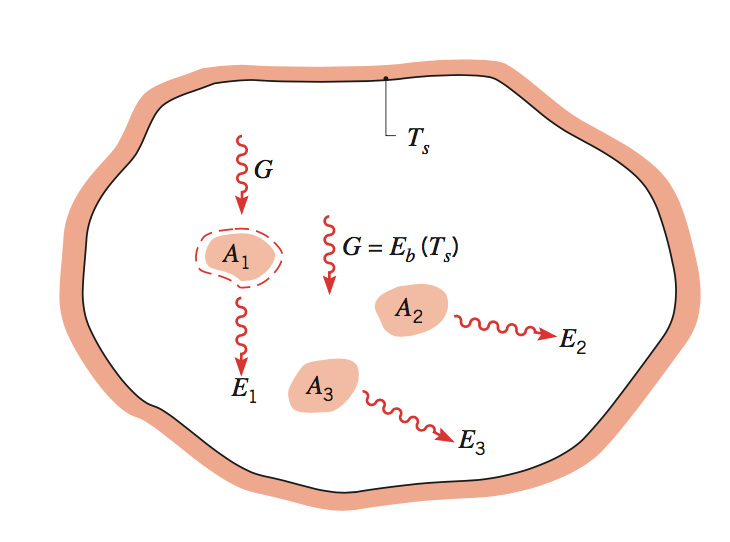
\includegraphics[width=1\textwidth]{fig14.png}\\
    \centering \small From Bergman et al. (2011)
    \end{minipage}
    \end{column}
    \begin{column}{.6\textwidth}
    \begin{minipage}[c][0.8\textheight][c]{\linewidth}
   \begin{itemize}
   	\item consider a perfectly insulated enclosure having black walls
   	\item assume the system has reached thermodynamic equilibrium
   	\item radiation emitted by the system to the walls is absorbed and the same amount of radiation absorbed by the walls is also emitted
   \end{itemize}
      \end{minipage}
    \end{column}
  \end{columns} 
\end{frame}

%------------------------------------------------
\begin{frame}{Kirchhoff's Law}
\begin{columns}[T]
    \begin{column}{.4\textwidth}
    \begin{minipage}[c][0.8\textheight][c]{\linewidth}
    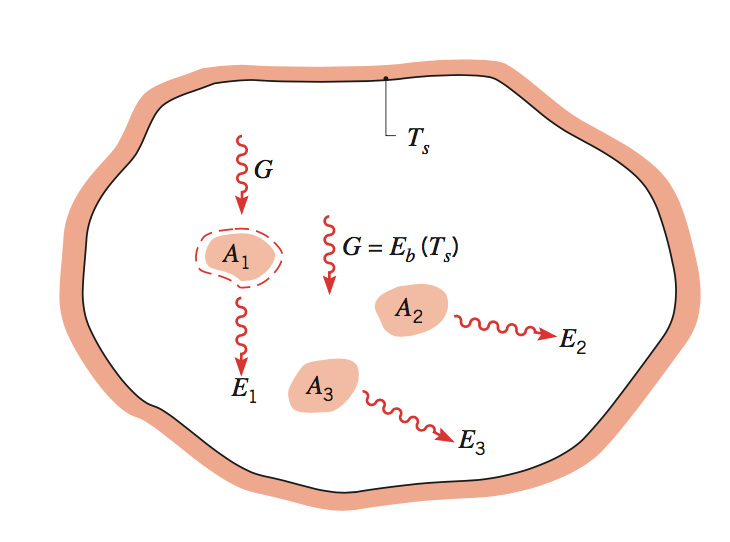
\includegraphics[width=1\textwidth]{fig14.png}\\
    \centering \small From Bergman et al. (2011)
    \end{minipage}
    \end{column}
    \begin{column}{.6\textwidth}
    \begin{minipage}[c][0.8\textheight][c]{\linewidth}
   \begin{itemize}
   	\item the emissivity of a given wavelength, $\epsilon_\lambda$ ($\frac{\text{emitting intensity}}{\text{Planck function}}$), of a medium is equal to the absorptivity, $A_\lambda$ ($\frac{\text{absorbed intensity}}{\text{Planck function}}$), of that medium under thermodynamic equilibrium
   	$$A_\lambda = \epsilon_\lambda = 1$$
   \end{itemize}
      \end{minipage}
    \end{column}
  \end{columns} 
\end{frame}

%------------------------------------------------
\begin{frame}{Kirchhoff's Law}
\begin{columns}[T]
    \begin{column}{.4\textwidth}
    \begin{minipage}[c][0.8\textheight][c]{\linewidth}
    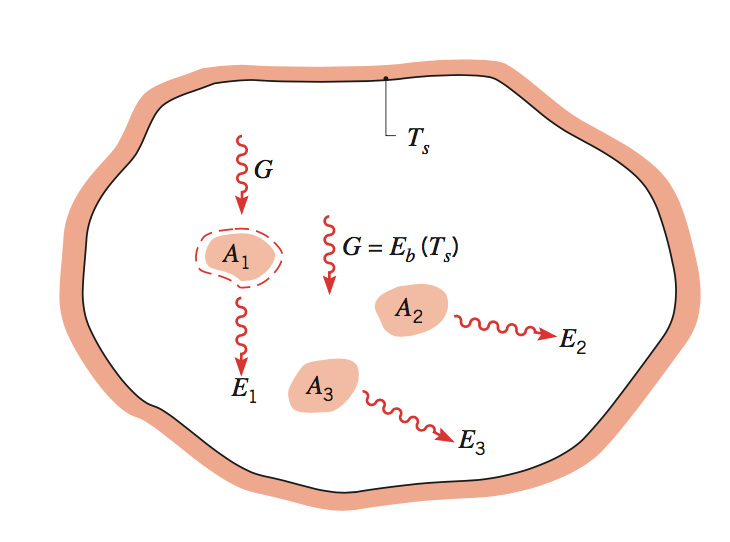
\includegraphics[width=1\textwidth]{fig14.png}\\
    \centering \small From Bergman et al. (2011)
    \end{minipage}
    \end{column}
    \begin{column}{.6\textwidth}
    \begin{minipage}[c][0.8\textheight][c]{\linewidth}
   \begin{itemize}
   	\item It can be shown that each of the confined bodies in the enclosure must adhere to:
   	$$\frac{E_1(T_s)}{A_{\lambda1}} = \frac{E_2(T_s)}{A_{\lambda2}} = \ldots = E_b(T_s)$$
   	\item since $A_\lambda \le 1$, $E(T_s) \le E_b(T_s)$
   	\item no real surface can have an emissive power exceeding that of a black surface at the same temperature
   	\item thus, a blackbody is confirmed to be a perfect emitter
   \end{itemize}
      \end{minipage}
    \end{column}
  \end{columns} 
\end{frame}


%------------------------------------------------
\section{Heat Transfer in Soils and Other Materials} %
%------------------------------------------------
\framecard[colorred]{{\color{white}\Huge Introduction to Heat Transfer\\~\\in Soils and Other Materials}}
%------------------------------------------------
\begin{frame}{Surface/Skin Temperature}
\begin{fancydefs}
	$T_s$  - The temperature at the air-soil interface.
\end{fancydefs}
An ``ideal'' surface has uniform $T_s$ and varies in time in response to energy fluxes at the surface. Inhomogeneous surfaces are likely to have spatially varying surface temperatures. 
~\\~\\
$T_s$ depends on
\begin{itemize}
	\item radiation balance
	\item surface exchange processes (\textit{e.g.}, turbulence)
	\item vegetative cover
	\item thermal properties of the subsurface
\end{itemize}
\end{frame}

%------------------------------------------------
\begin{frame}{Surface/Skin Temperature}
Data from MATERHORN field campaign for a playa site at the U.S. Army Dugway Proving Grounds. Note the large surface temperature heterogeneities
\begin{figure}
	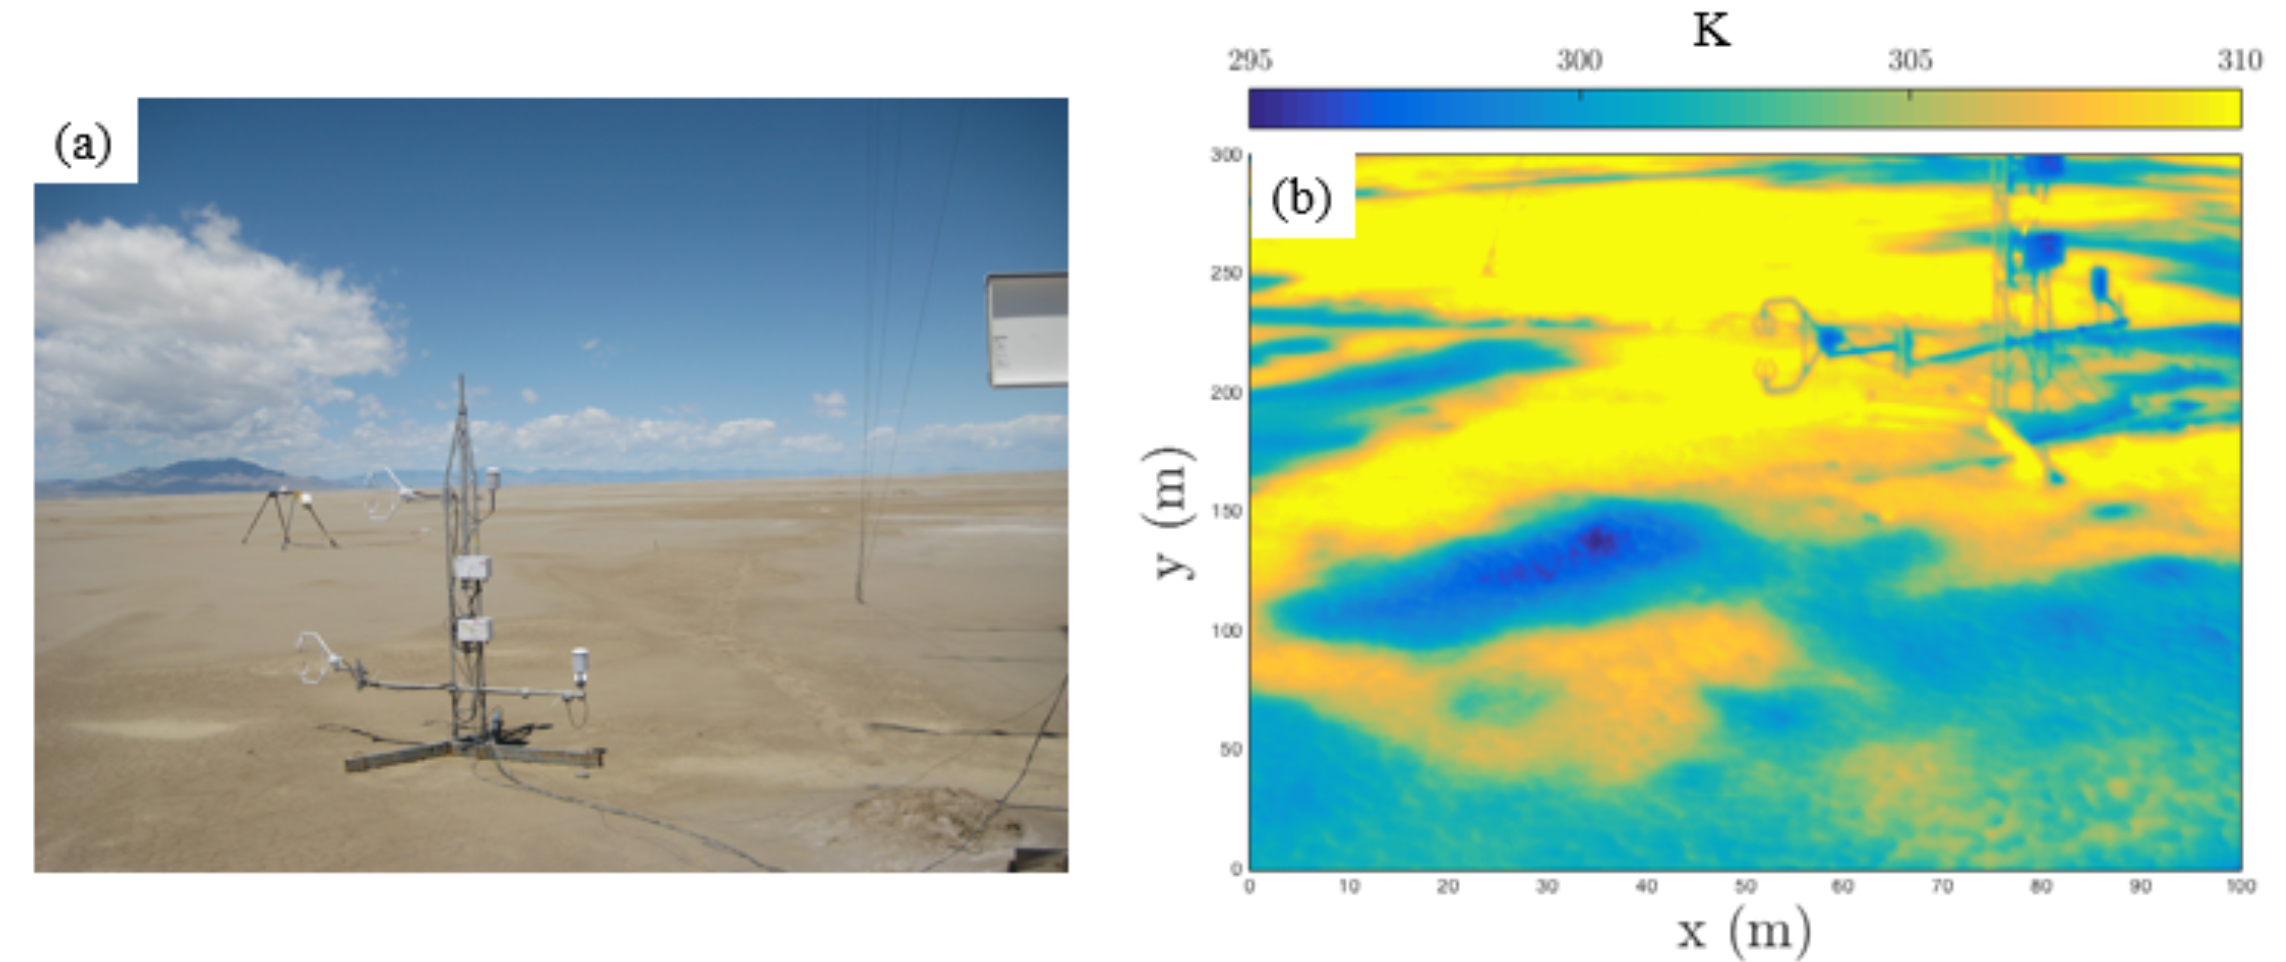
\includegraphics[width=\textwidth]{fig15.png}
	\newline \centering \tiny figure courtesy Travis Morrison
\end{figure}
\end{frame}

%------------------------------------------------
\begin{frame}{Surface/Skin Temperature}
\begin{fancydefs}
	$T_s$  - The temperature at the air-soil interface.
\end{fancydefs}
$T_s$ is difficult to measure
\begin{itemize}
	\item very large temperature gradients near the surface both in the air and soil ($10-20\ \kelvin\ \milli\reciprocal\metre$ possible in air above bare heated soil!)
	\item usually computed by extrapolating air/soil temperatures
	\item radiometer - uses $R_{L\uparrow} \sim -\epsilon \sigma T_s^4$ (Stefan-Boltzman Law)
\end{itemize}
%\begin{figure}
%	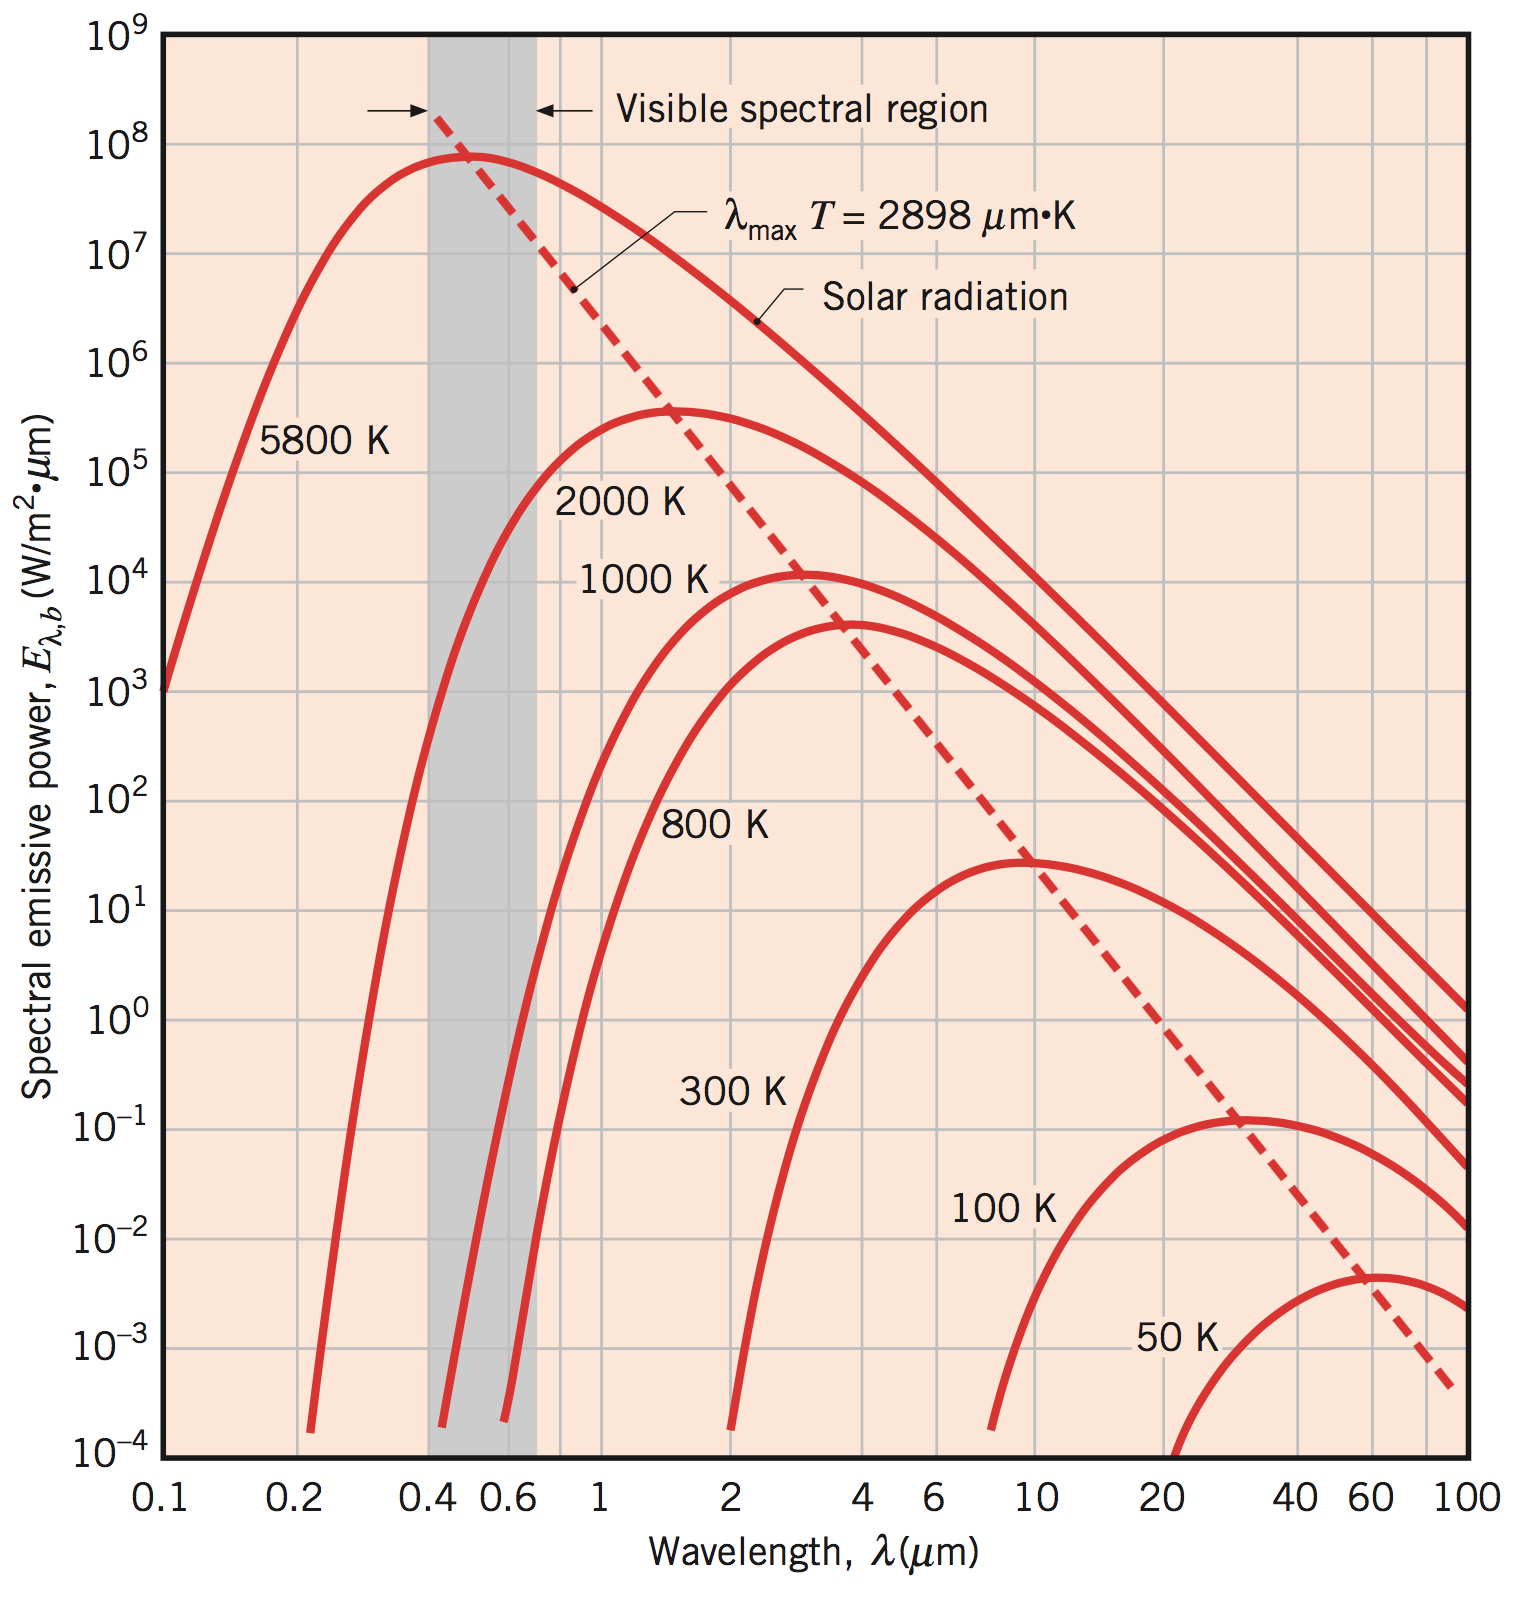
\includegraphics[width=\textwidth]{fig1.png}
%	\newline \centering \tiny figHoch et al. (2014)
%\end{figure}
\end{frame}
%------------------------------------------------
\begin{frame}{Surface/Skin Temperature}

{\large \textbf{Diurnal Range}}
\begin{itemize}
	\item in a dry desert: $\sim$ $40$-$50$\ $\celsius$ 
	\item Surface and subsurface moisture moderate the range
	\begin{itemize}
		\item increased evaporation from the surface
		\item increased heat capacity ($c$) and conductivity of the soil ($k$)
		\item wet soils may dry changing the temperature response
	\end{itemize}
	\item Vegetation moderates diurnal range moderate the range
	\begin{itemize}
		\item intercepts incoming solar radiation $\rightarrow$ lower surface temps during the day
		\item intercepts outgoing longwave radiation
		\item enhanced latent heat flux due to evapotranspiration (ET) 
		\item increased turbulence
	\end{itemize}
\end{itemize}
\end{frame}

%------------------------------------------------
\begin{frame}{Diurnal Soil and  Temperature}
\begin{itemize}
	\item On a clear day, the max surface temperature is generally reached about 1-2 hours after peak incoming solar radiation (insolation; solar noon)
	\item The min surface temperature occurs in the early morning hours
	\item On a larger scale, this is why the maximum annual temperatures (northern hemisphere) are not reached in June even though this time has peak insolation
\end{itemize}
\end{frame}

%------------------------------------------------
\begin{frame}{Diurnal Soil and  Temperature}
\begin{figure}
	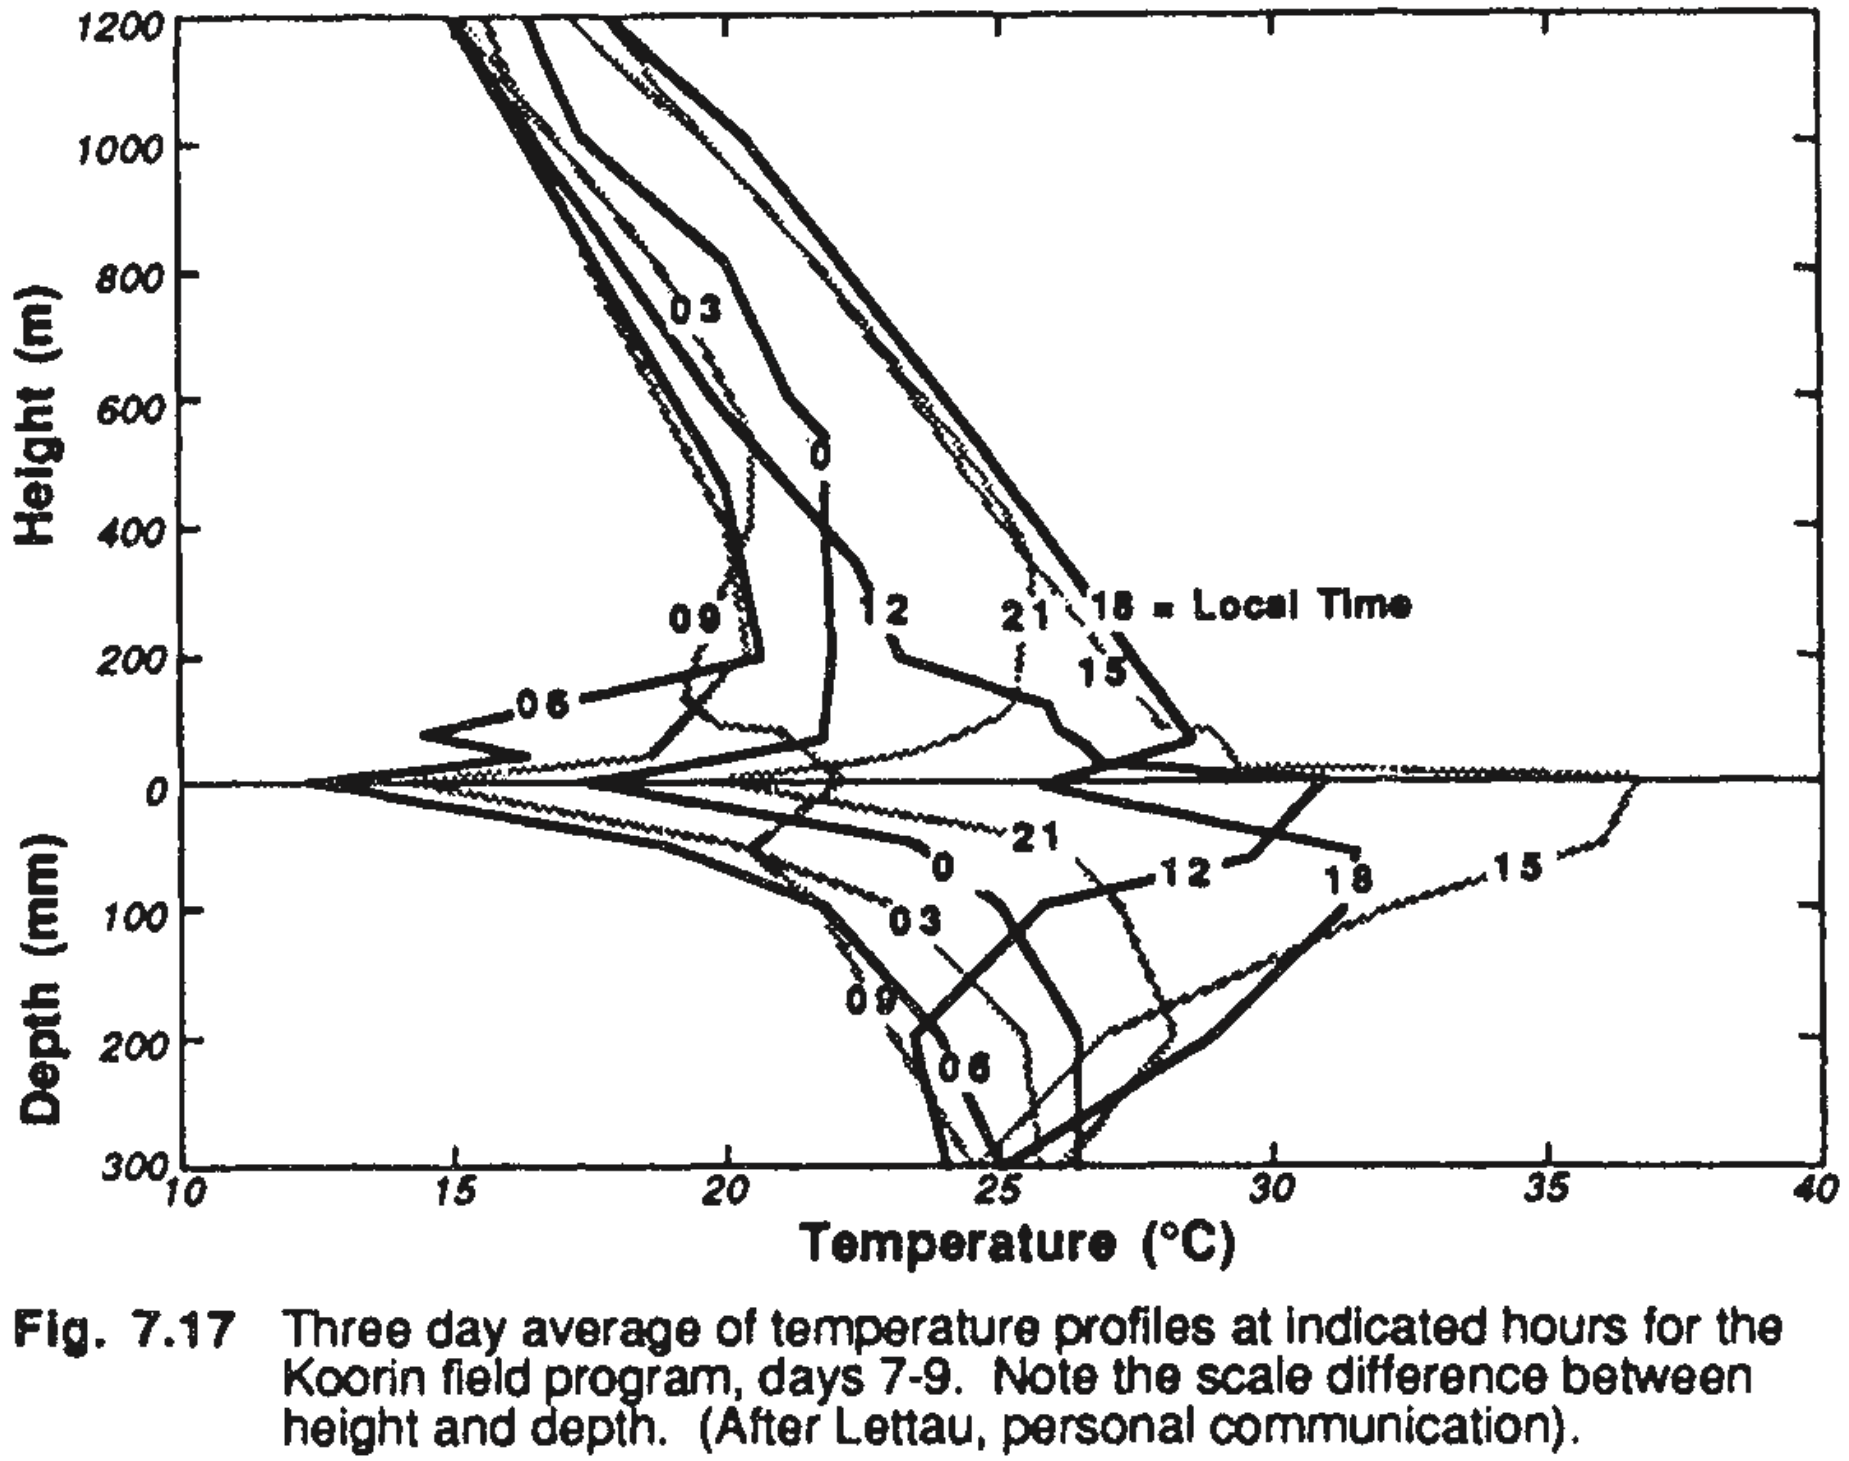
\includegraphics[width=0.9\textwidth]{fig2.png}
	\newline \centering \tiny Stull (1988)
\end{figure}
\end{frame}


%------------------------------------------------

\begin{frame}{Hysteresis}
\begin{columns}[T]
    \begin{column}{.35\textwidth}
    \begin{minipage}[c][0.8\textheight][c]{\linewidth}
    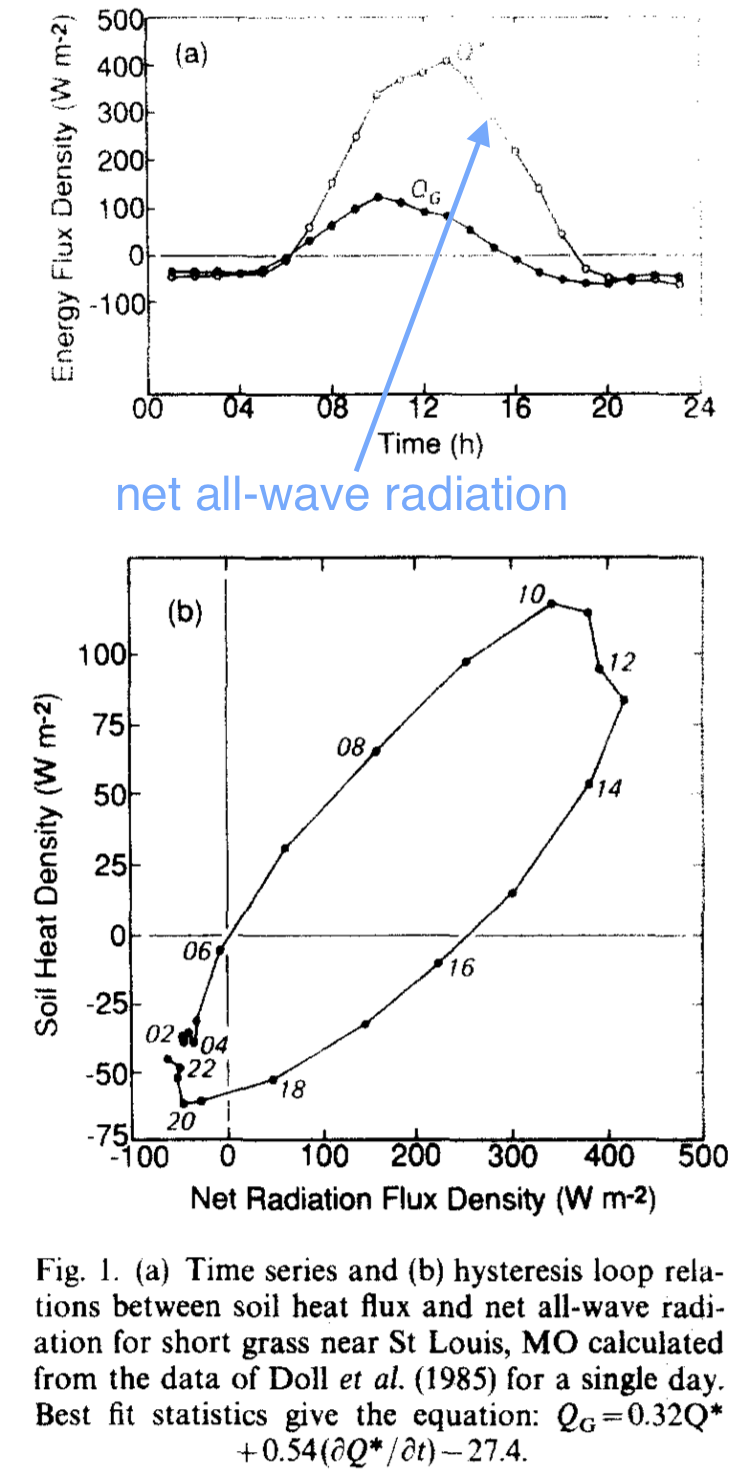
\includegraphics[width=1\textwidth]{fig12.png}
    \end{minipage}
    \end{column}
    \begin{column}{.65\textwidth}
    \begin{minipage}[c][1\textheight][c]{\linewidth}
    {\large \textbf{hysteresis}}\\
    \begin{fancydefs}
    	the phenomenon in which the value of a physical property lags behind changes in the effect causing it\\~\\the dependence of the state of a system on its history
    \end{fancydefs}
    $$\Delta H_s = \int \frac{\partial (\rho C T)}{\partial t} dz$$
      \end{minipage}
    \end{column}
  \end{columns} 
\end{frame}

%------------------------------------------------
\begin{frame}{Sub-surface Soil Temperature}

\begin{itemize}
	\item much easier to measure - thermocouple
	\item amplitude of the temperature fluctuations decrease exponentially with depth 
	\item depends on:
	\begin{itemize}
		\item latitude
		\item time of year
		\item net radiation
		\item soil texture (porosity) and moisture content
		\item ground cover
		\item surface weather conditions
	\end{itemize}
\end{itemize}
\end{frame}

%------------------------------------------------
\begin{frame}{Thermal Properties of Soil}

\begin{itemize}
	\item \underline{Specific Heat} - $c$ ($\joule\  \kilo\reciprocal\gram\ \reciprocal\kelvin$) - the amount of heat absorbed by a material to raise the temperature of a unit mass of material by 1$\kelvin$
	\item \underline{Thermal Conductivity} - $k$ ($\watt\ \reciprocal\metre\ \reciprocal\kelvin$) - material property; the ability of a material to conduct heat
	\item \underline{Thermal Diffusivity} - $\alpha_h$ ($\square\metre\ \reciprocal\second$) - ratio of thermal conductivity to heat capacity
\end{itemize}
\end{frame}

%------------------------------------------------

\begin{frame}{Thermal Properties of Soil}
\begin{columns}[T]
    \begin{column}{.45\textwidth}
    \begin{minipage}[c][0.8\textheight][c]{\linewidth}
    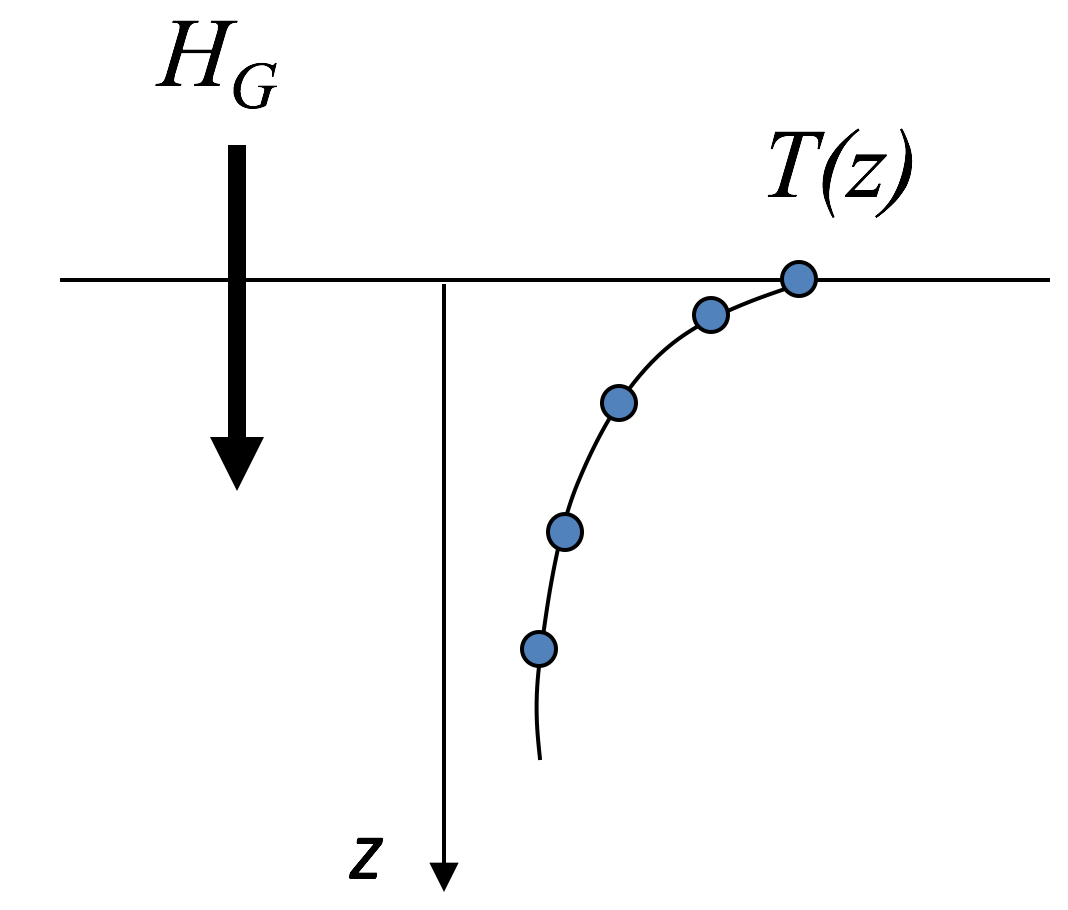
\includegraphics[width=1\textwidth]{fig5.png}
    \end{minipage}
    \end{column}
    \begin{column}{.55\textwidth}
    \begin{minipage}[c][0.8\textheight][c]{\linewidth}
    {\large \textbf{1D Thermal Conduction}}
    \begin{align*}
    	H_G &= -k\frac{\partial T}{\partial z}\quad \parbox{8em}{Fourier's \\conduction law}\\
    	\alpha_h &= \underbrace{\frac{k}{\boxed{\rho c}} = \frac{k}{\boxed{C}}}_{\text{soil heat capacity}}\\
    	\frac{\partial (\rho cT)}{\partial t} &= -\frac{\partial H_G}{\partial z}\\
    	\frac{\partial (\rho cT)}{\partial t} &= k\frac{\partial^2 T}{\partial z^2}\\
    	\Aboxed{\frac{\partial T}{\partial t} &= \alpha_h\frac{\partial^2 T}{\partial z^2}}
    \end{align*}
      \end{minipage}
    \end{column}
  \end{columns} 
\end{frame}
%------------------------------------------------
\begin{frame}{Solutions}
$$\frac{\partial T}{\partial t} = \alpha_h\frac{\partial^2 T}{\partial z^2}$$
\begin{itemize}
	\item analytical - multiple methods
	\item numerical - \textit{e.g.}, finite difference
	\item force-restore - 2 layer slab model (see Stull Ch.7, Blackadar 1976) 
\end{itemize}
\end{frame}

%------------------------------------------------
\begin{frame}{Diurnal and Annual Soil Temperature Temporal Variability}

\begin{figure}
	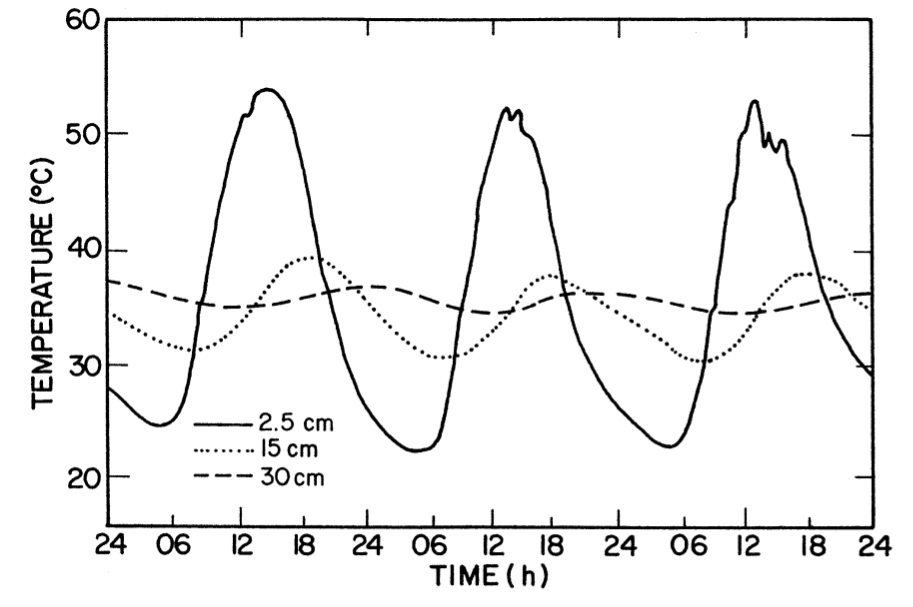
\includegraphics[width=0.5\textwidth]{fig3}
	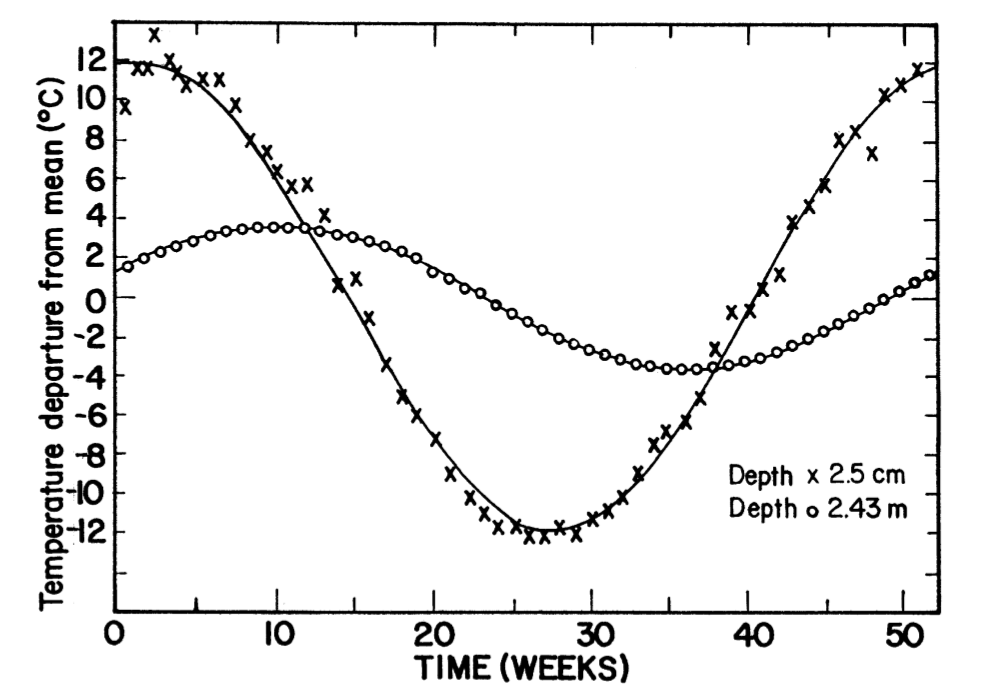
\includegraphics[width=0.48\textwidth]{fig4}
	\caption{{\large \textbf{diurnal wave}} (left), 	{\large \textbf{annual wave} (right)}}
\end{figure}
\end{frame}
%------------------------------------------------

\begin{frame}{Soil Heat Transfer}
\begin{columns}[T]
    \begin{column}{.4\textwidth}
    \begin{minipage}[c][0.8\textheight][c]{\linewidth}
    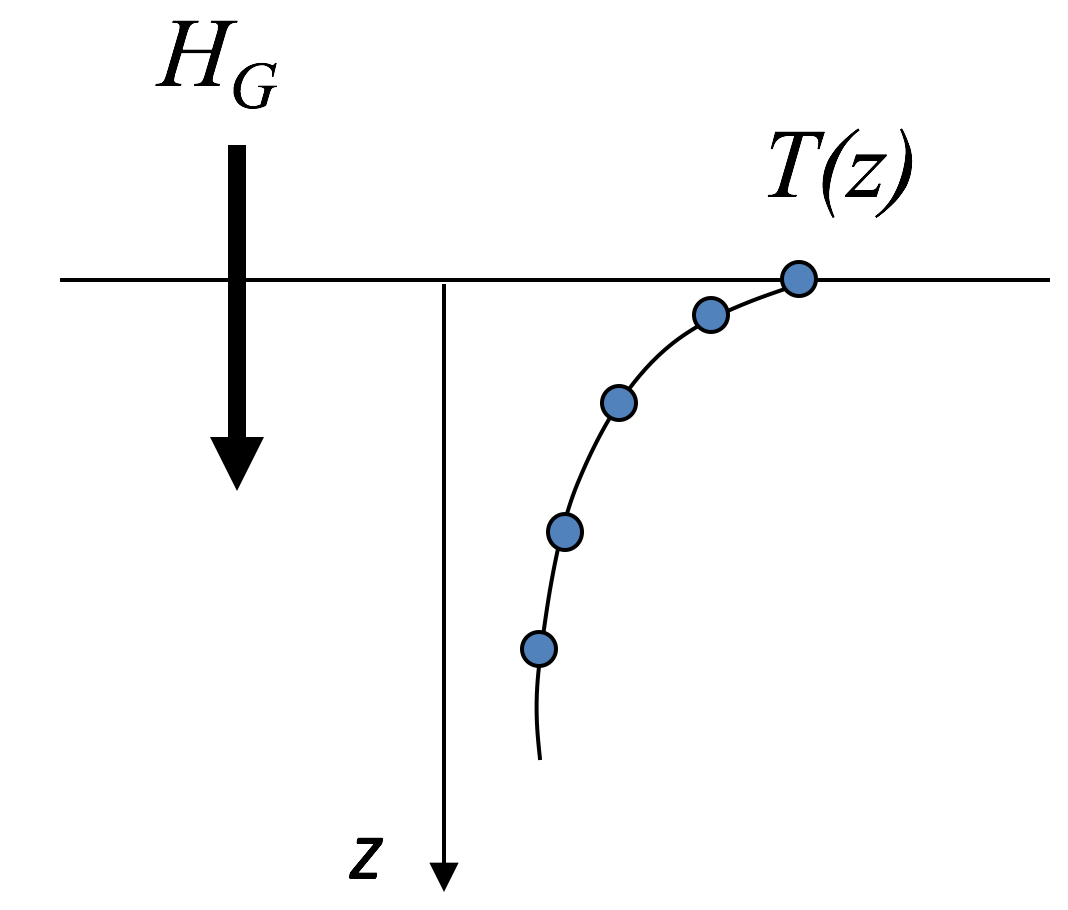
\includegraphics[width=1\textwidth]{fig5.png}
    \end{minipage}
    \end{column}
    \begin{column}{.6\textwidth}
    \begin{minipage}[c][0.8\textheight][c]{\linewidth}
    {\large \textbf{1D Thermal Conduction}}
    $$\frac{\partial (CT)}{\partial t} = -\frac{\partial H}{\partial z}$$
    $$H(z=0) - H(z=D) = \int^{z=D}_{z=0} \frac{\partial (CT)}{\partial t} dz$$
    $$\underbrace{H_G}_{\substack{\text{ground}\\\text{heat flux}}} = \underbrace{H_D}_{\substack{\text{reference}\\\text{depth}}} + \underbrace{\int^{z=D}_{z=0} \frac{\partial (CT)}{\partial t} dz}_{\text{storage}}$$
      \end{minipage}
    \end{column}
  \end{columns} 
\end{frame}

%------------------------------------------------

\begin{frame}{Soil Heat Transfer: Governing Parameters}
\begin{itemize}
	\item thermal conductivity - $k$
	\item heat cpacity - $C_s$
	\item thermal diffusivity - $\alpha$ (sometimes $\kappa$)
	\item thermal admittance - $\mu$	
\end{itemize}
\end{frame}

%------------------------------------------------

\begin{frame}{Soil Heat Transfer: Governing Parameters}

{\large \textbf{thermal conductivity} $k$ ($\watt\ \reciprocal\metre\ \reciprocal\kelvin$})
\begin{itemize}
	\item the ability of a material to conduct heat
	\item depends on:
	\begin{itemize}
		\item soil particles
		\item soil porosity
		\item moisture content
	\end{itemize}
\end{itemize}
\end{frame}

%------------------------------------------------

\begin{frame}{Soil Heat Transfer: Governing Parameters}

{\large \textbf{heat capacity} $C_s = \rho c$ ($\joule\ \metre\rpcubed\ \reciprocal\kelvin$})
\begin{itemize}
	\item $c$ - specific heat of the soil ($\joule\ \kilo\reciprocal\gram\ \reciprocal\kelvin$)
	\item relates to the ability of a material to store heat
	\item the amount of heat ($\joule$) necessary to increase a unit volume ($\metre\cubed$) of a substance by $1\kelvin$
	\item water ($\sim 5\ \joule\ \metre\rpcubed\ \reciprocal\kelvin$) has a very high heat capacity, air is quite low
	\item Depends on:
	\begin{itemize}
		\item porosity
		\item mineral content
		\item organic content
		\item air, etc.
	\end{itemize}
\end{itemize}
\end{frame}

%------------------------------------------------

\begin{frame}{Soil Heat Transfer: Governing Parameters}

{\large \textbf{thermal diffusivity } $\alpha = k/C_s$ ($\metre\squared\ \reciprocal\second$})
\begin{itemize}
	\item Controls the speed at which temperature waves move through the soil and the depth of thermal influence of an active surface
	\item In other words, consider it to be the rate of transfer of heat in a material from the ``hot side'' to the ``cold side''
	\item water ($\sim 1.43\times 10^{-7}\ \metre\squared\ \reciprocal\second$)
	\item air ($\sim 1.9\times 10^{-5}\ \metre\squared\ \reciprocal\second$)
\end{itemize}
\end{frame}

%------------------------------------------------

\begin{frame}{Soil Heat Transfer: Governing Parameters}

{\large \textbf{thermal admittance } $\mu = \sqrt{kC_s}$ ($\joule\ \metre\rpsquared\ \second^{-1/2}\ \reciprocal\kelvin)$}
\begin{itemize}
	\item a surface property - not a soil property
	\item the ability of a surface to accept or release heat
	\item high $\mu$ - metals
	\item low $\mu$ - wood
	\item high $\mu$ materials feel cooler to the touch even though they have the same surface temperature
\end{itemize}
\end{frame}

%------------------------------------------------

\begin{frame}{Soil Heat Transfer: Governing Parameters Typical Values}

\begin{figure}
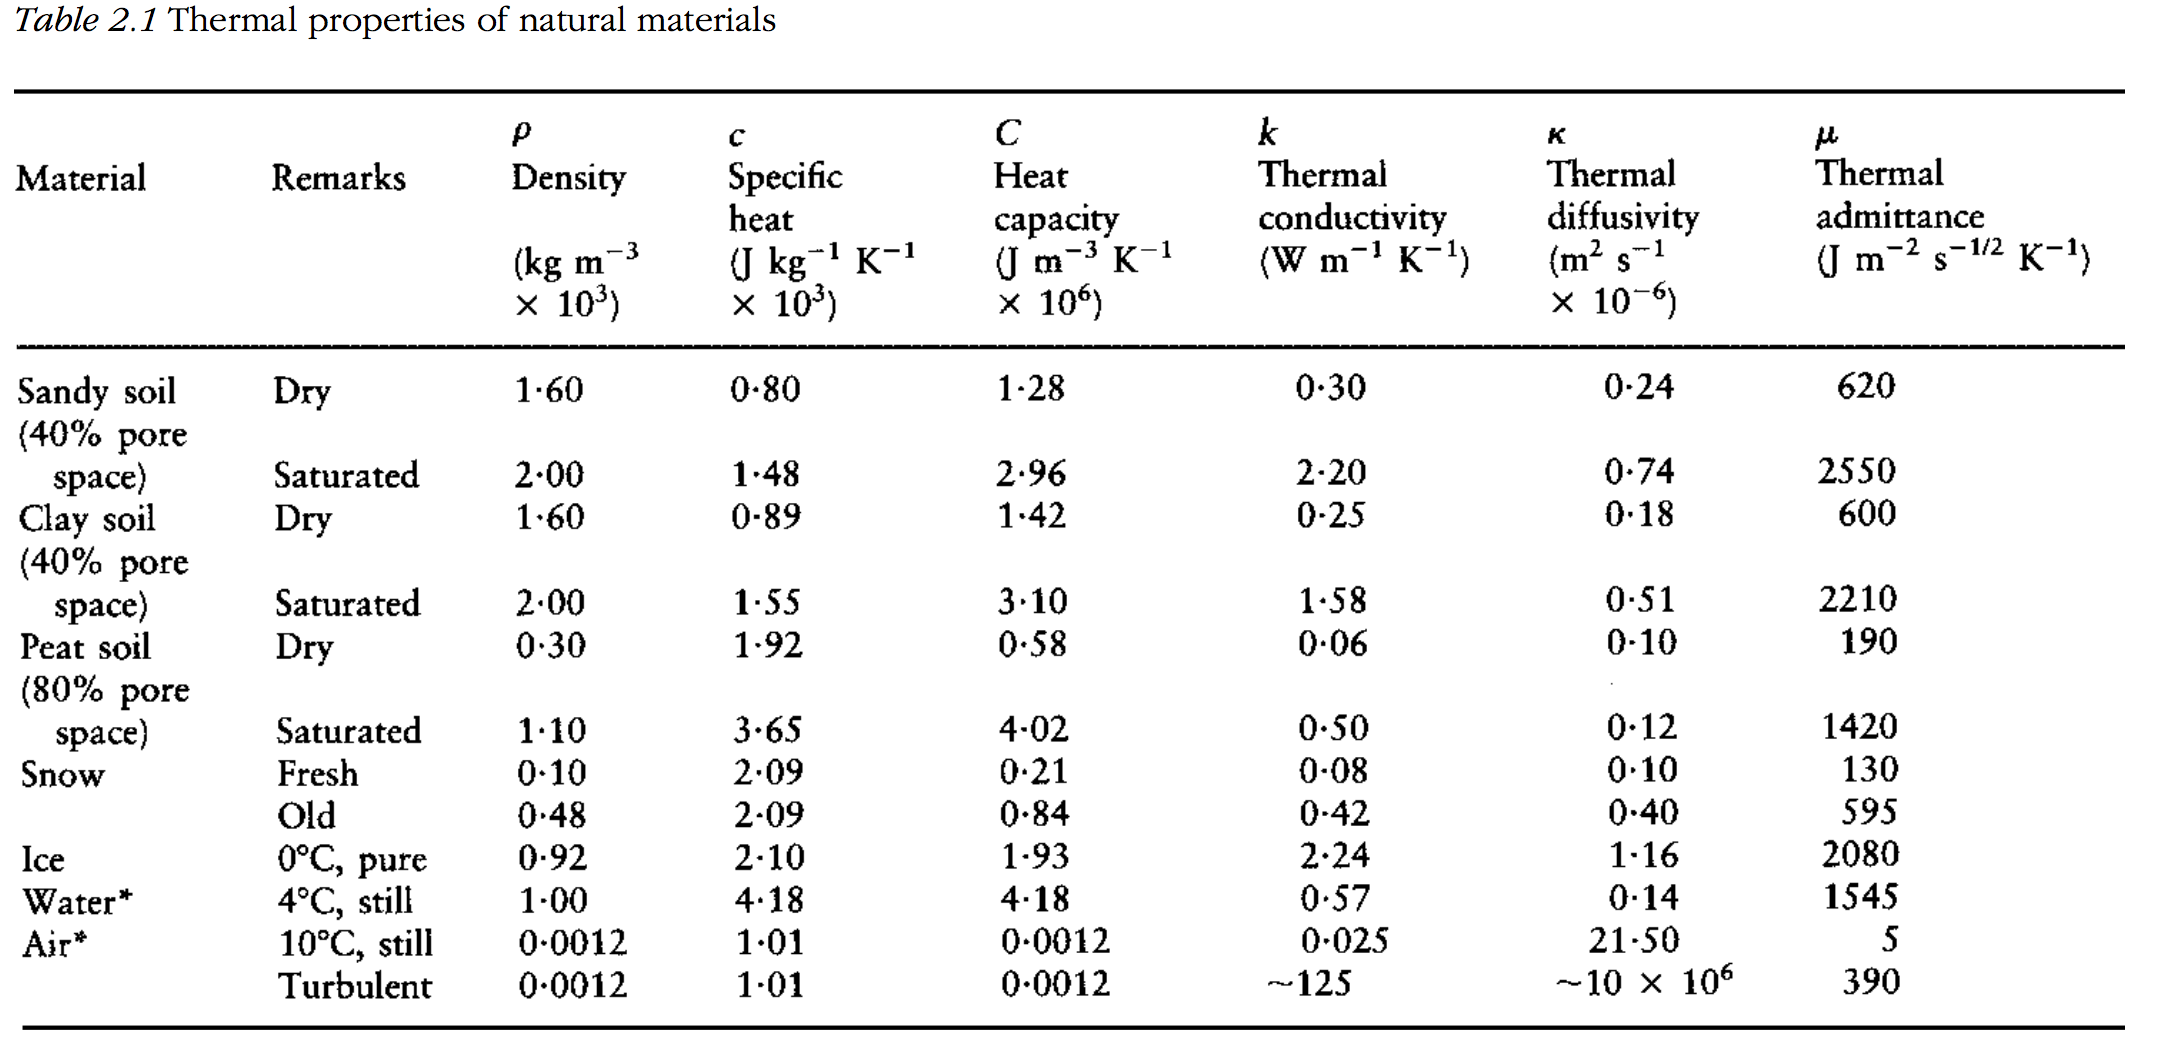
\includegraphics[width=\textwidth]{fig6}
\centering \tiny~\\Oke (1987)
\end{figure}
\end{frame}

%------------------------------------------------

\begin{frame}{Effect of Soil Moisture on Thermal Properties}

\begin{figure}
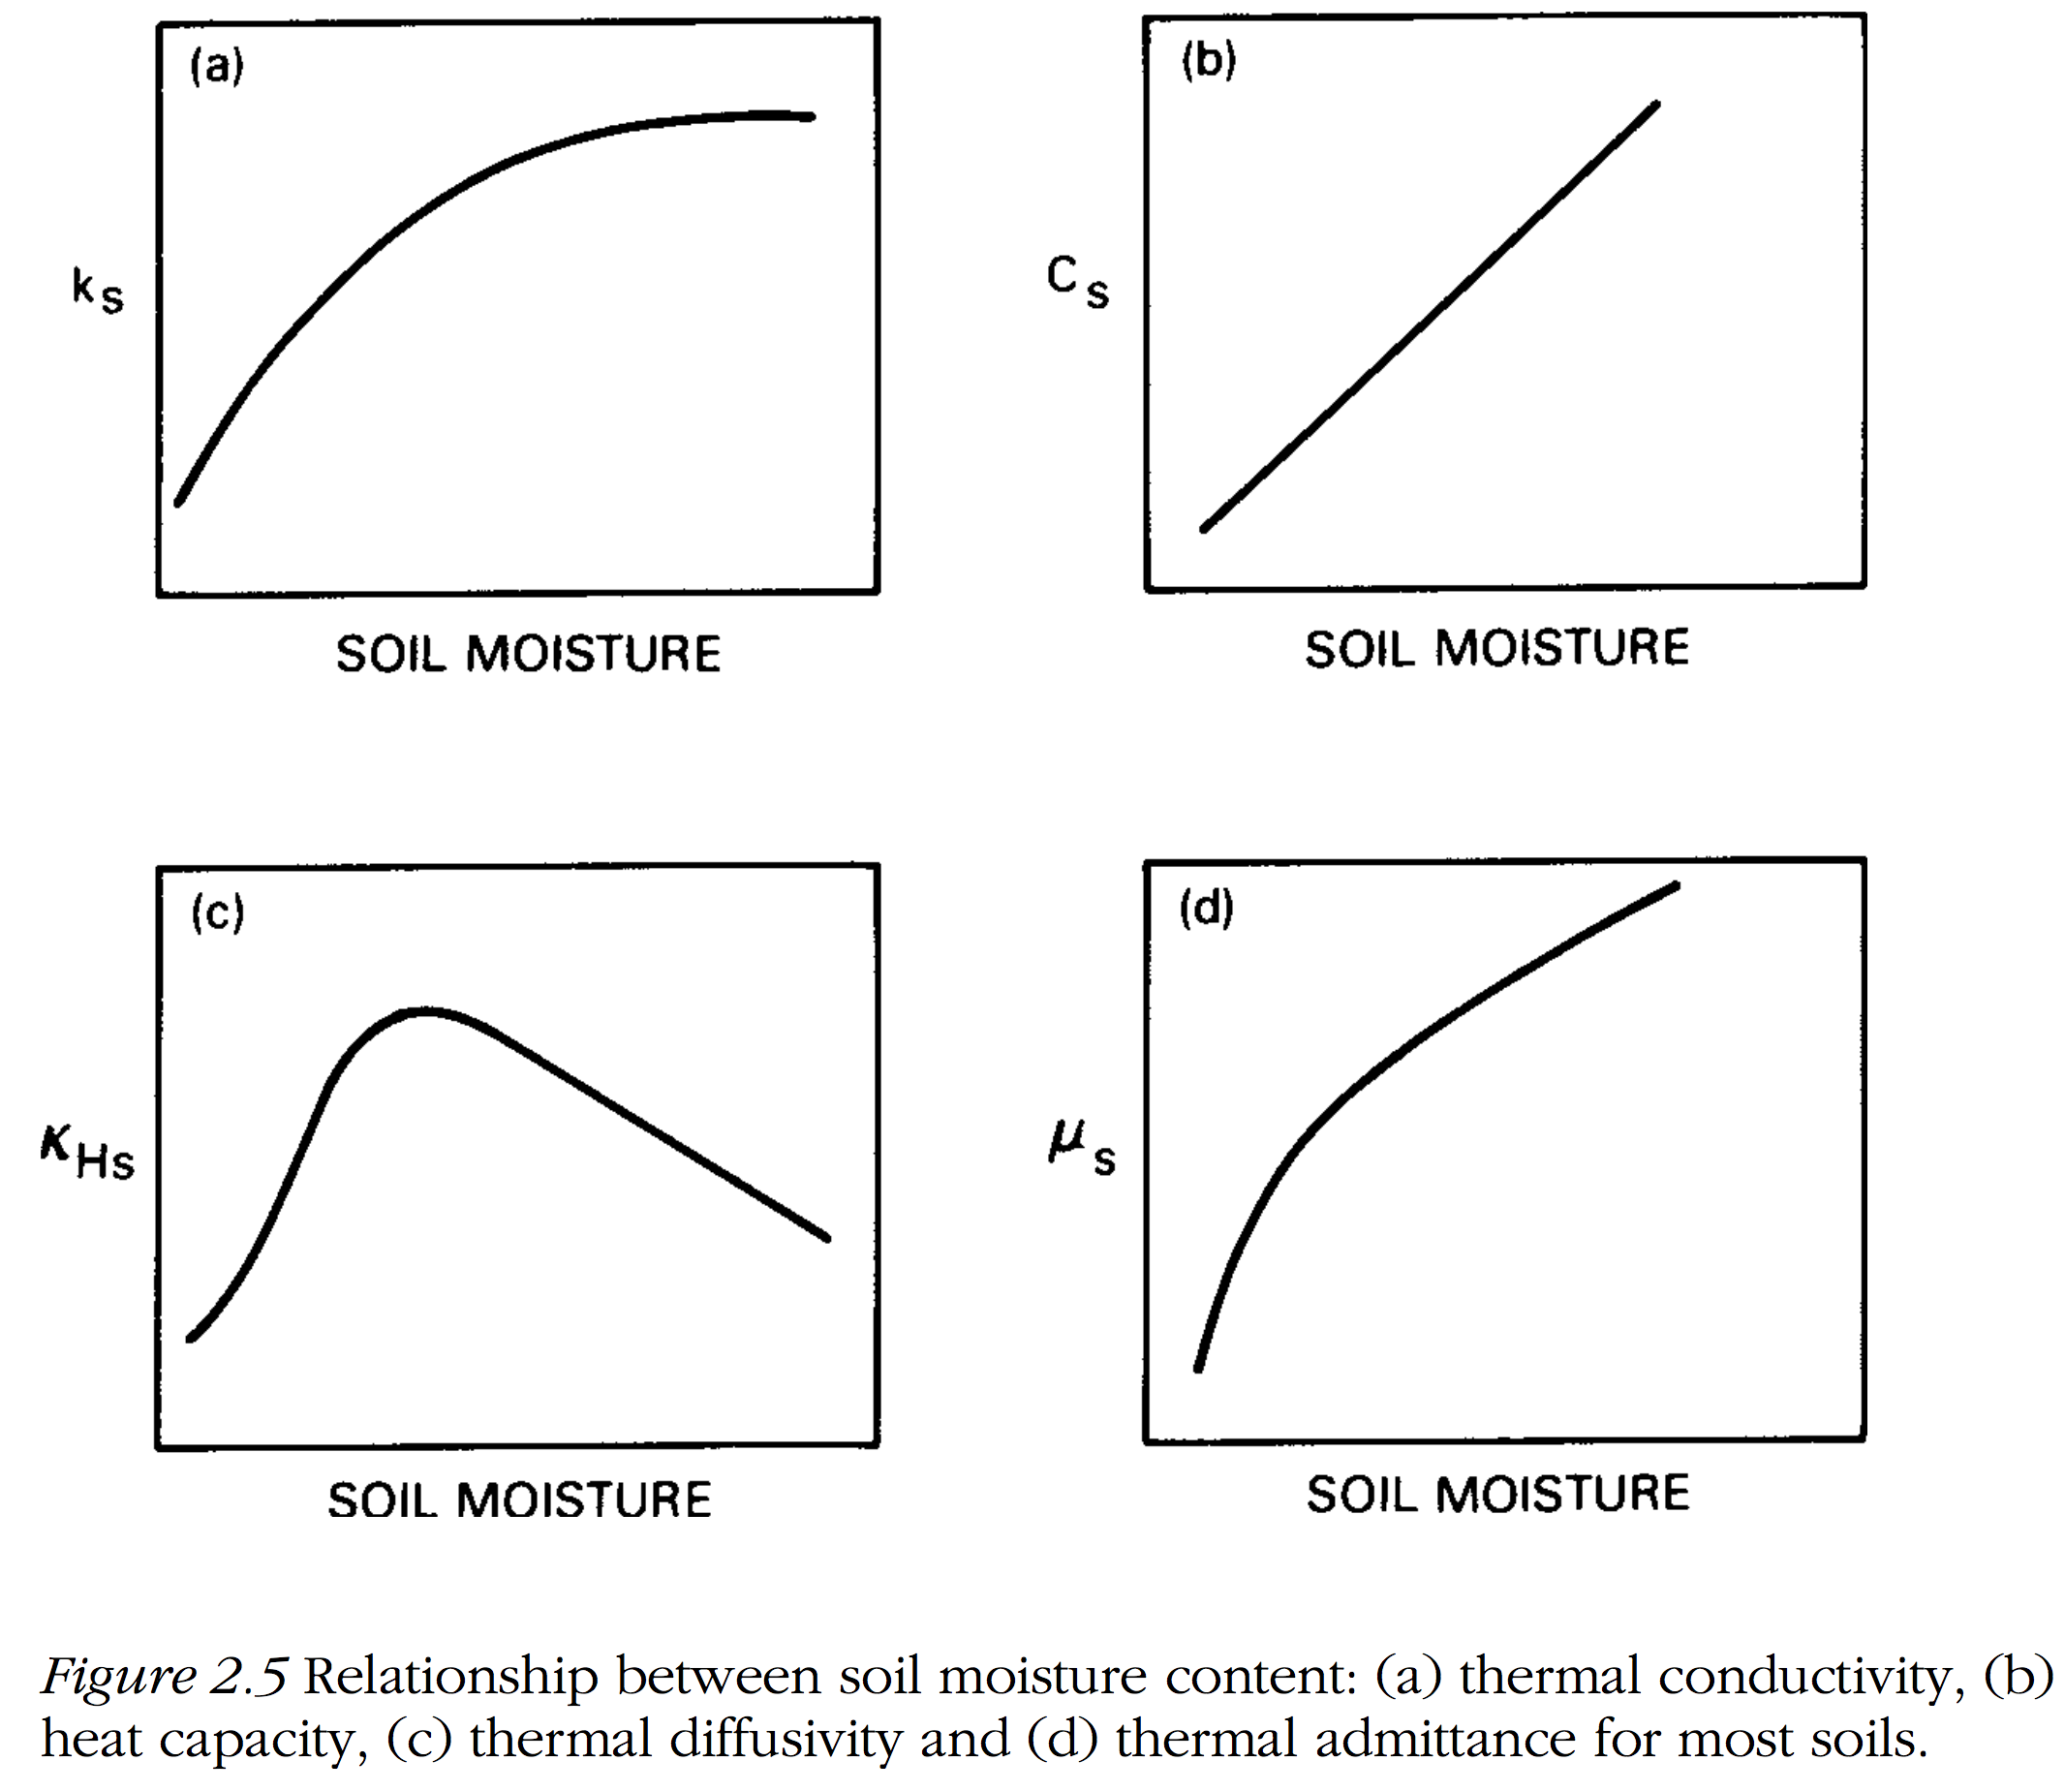
\includegraphics[width=0.88\textwidth]{fig7}
\centering \tiny~\\Oke (1987)
\end{figure}
\end{frame}

%------------------------------------------------

\begin{frame}{Variation of Fluxes in Urban Areas}

\begin{figure}
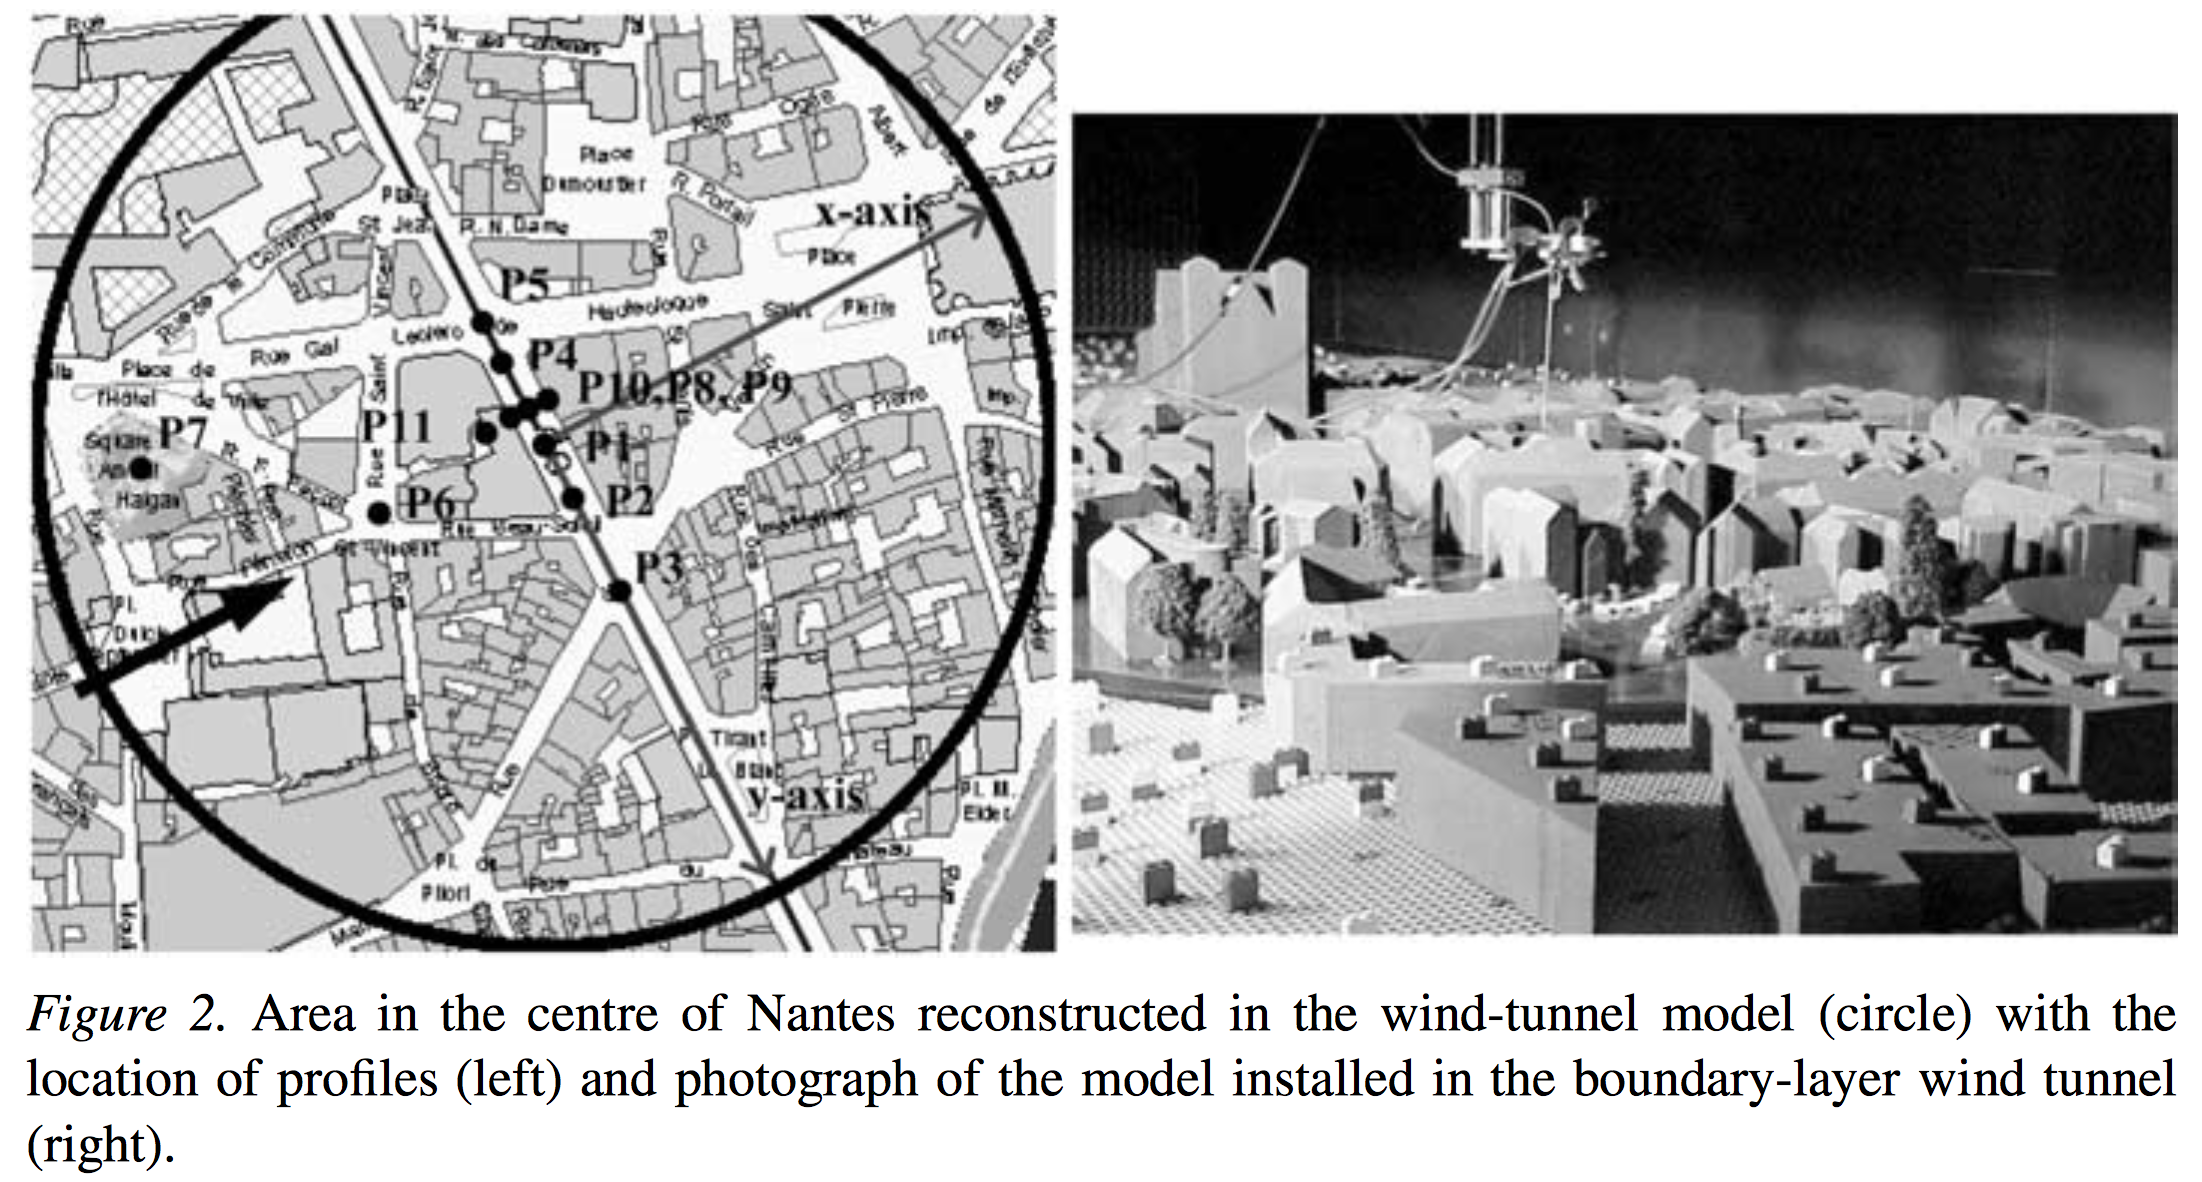
\includegraphics[width=\textwidth]{fig8}
\centering \tiny~\\From Kastner-Klein, P., and Rotach, M. W. (2004). Mean Flow and Turbulence Characteristics in an Urban Roughness Sublayer. Boundary-Layer Meteorology, 111(1), 55–84. 
\end{figure}
\end{frame}

%------------------------------------------------

\begin{frame}{Variation of Fluxes in Urban Areas}

\begin{figure}
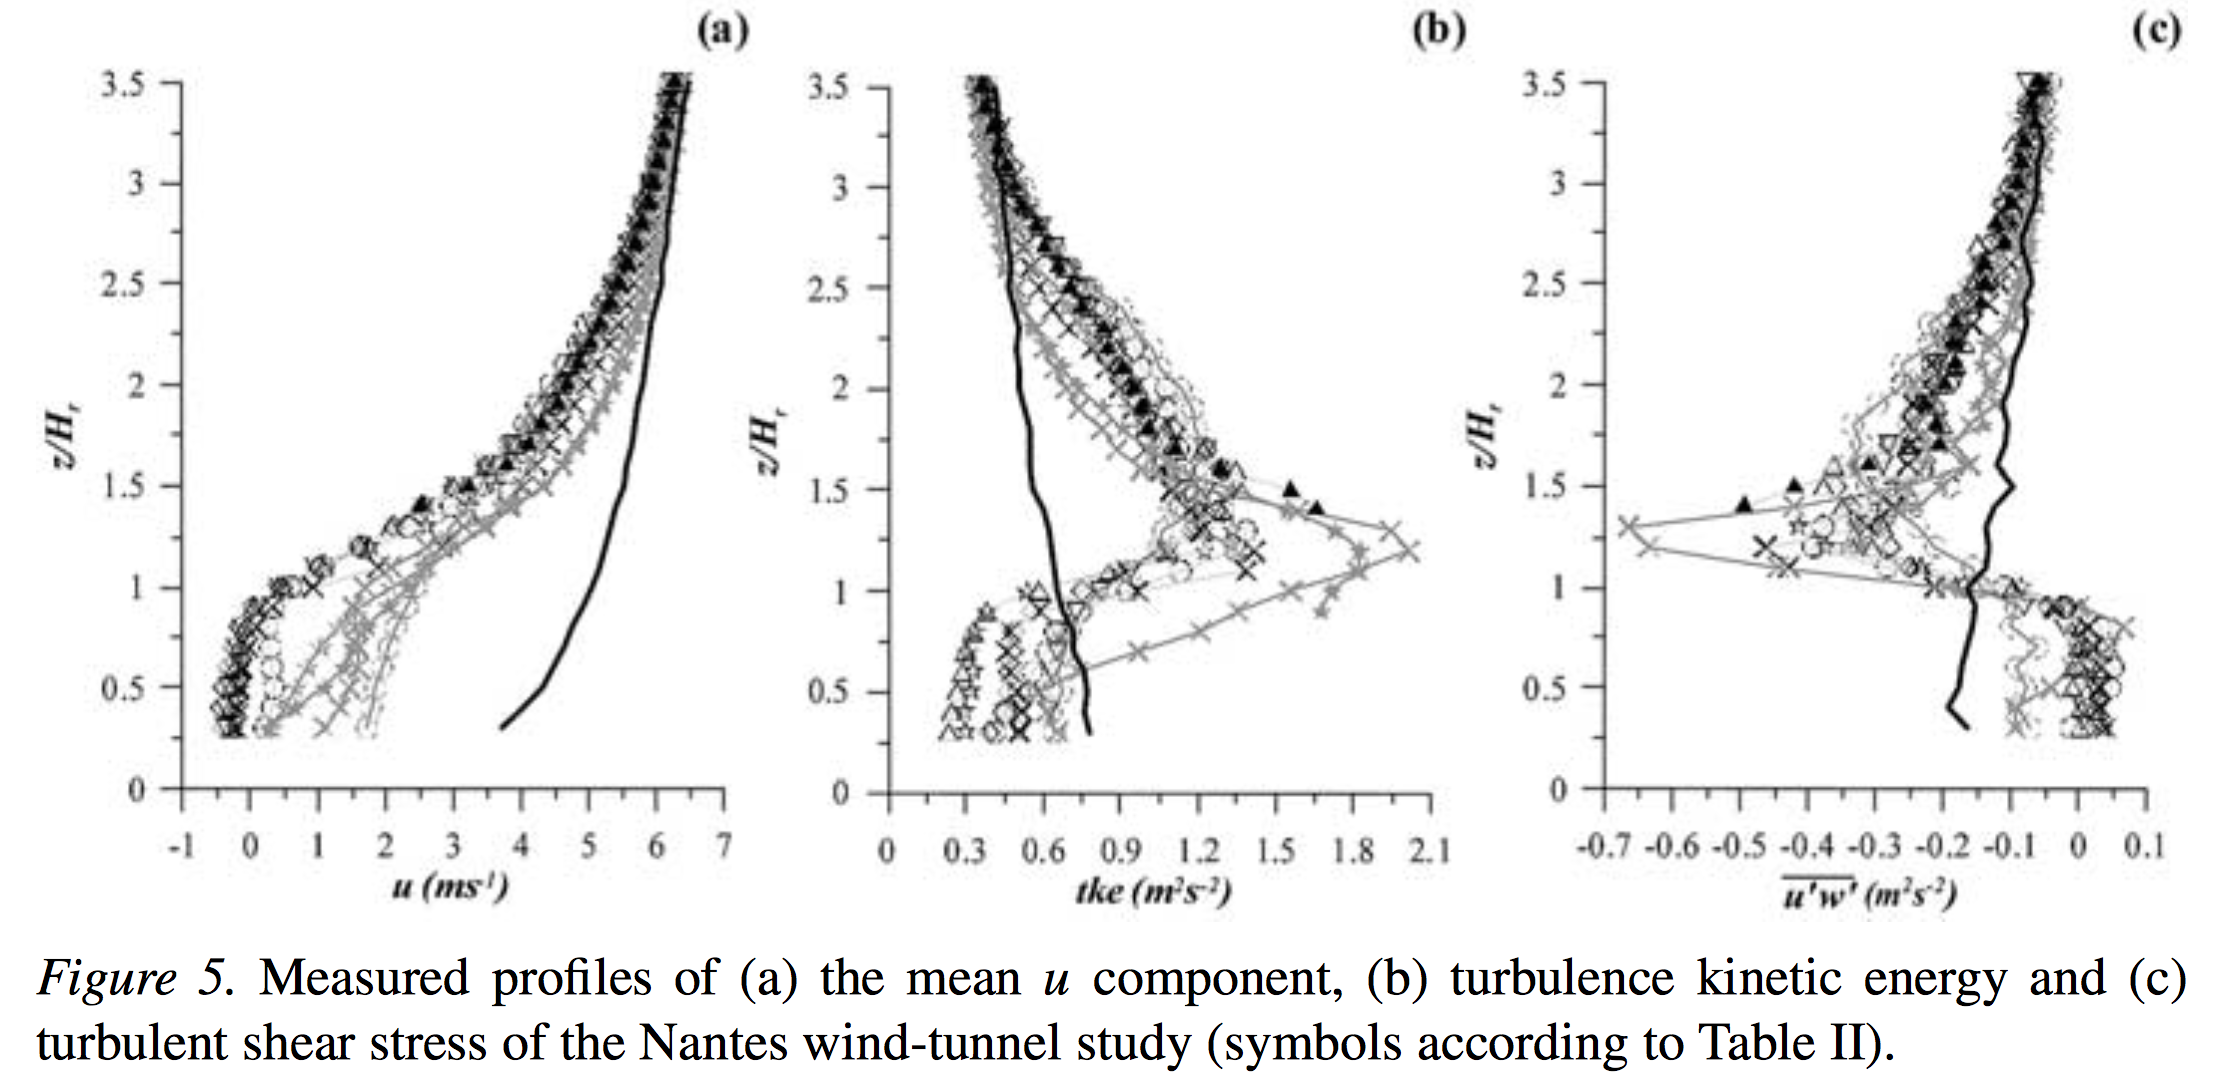
\includegraphics[width=\textwidth]{fig9}
\centering \tiny~\\From Kastner-Klein, P., and Rotach, M. W. (2004). Mean Flow and Turbulence Characteristics in an Urban Roughness Sublayer. Boundary-Layer Meteorology, 111(1), 55–84. 
\end{figure}
\end{frame}


%------------------------------------------------

\begin{frame}{Urban Areas}

\begin{figure}
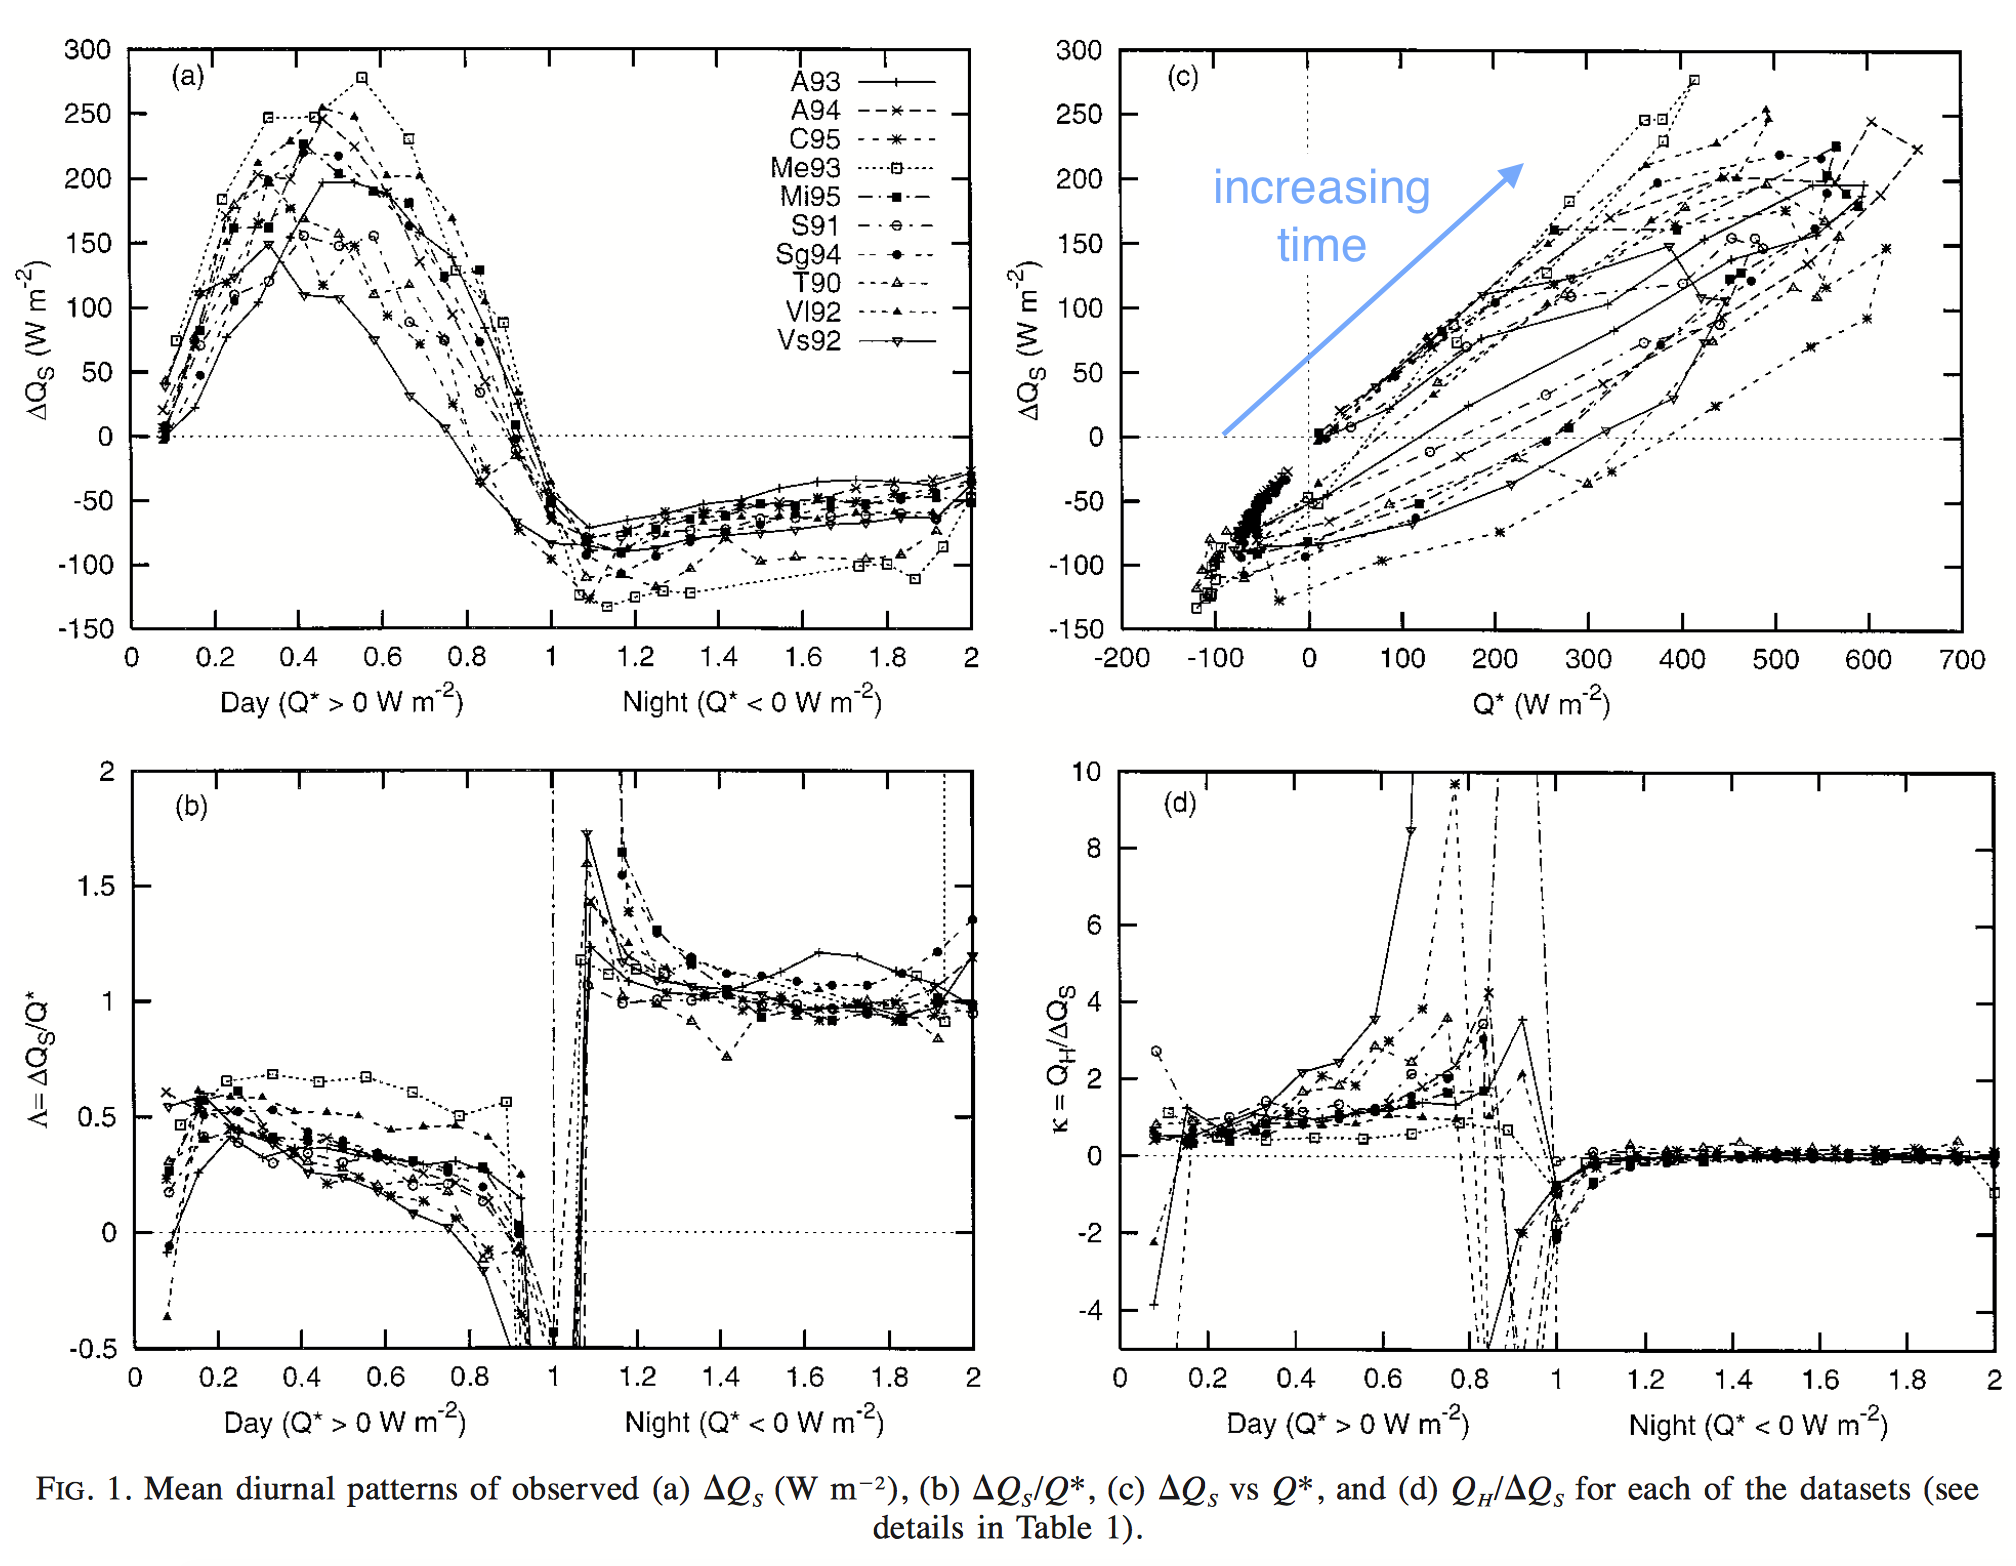
\includegraphics[width=0.8\textwidth]{fig10}
\centering \tiny~\\From Grimmond and Oke (1999) 
\end{figure}
More energy is transferred to the ``urban fabric'' in the morning - asymmetry
\end{frame}

%------------------------------------------------

\begin{frame}{Urban Areas}

\begin{figure}
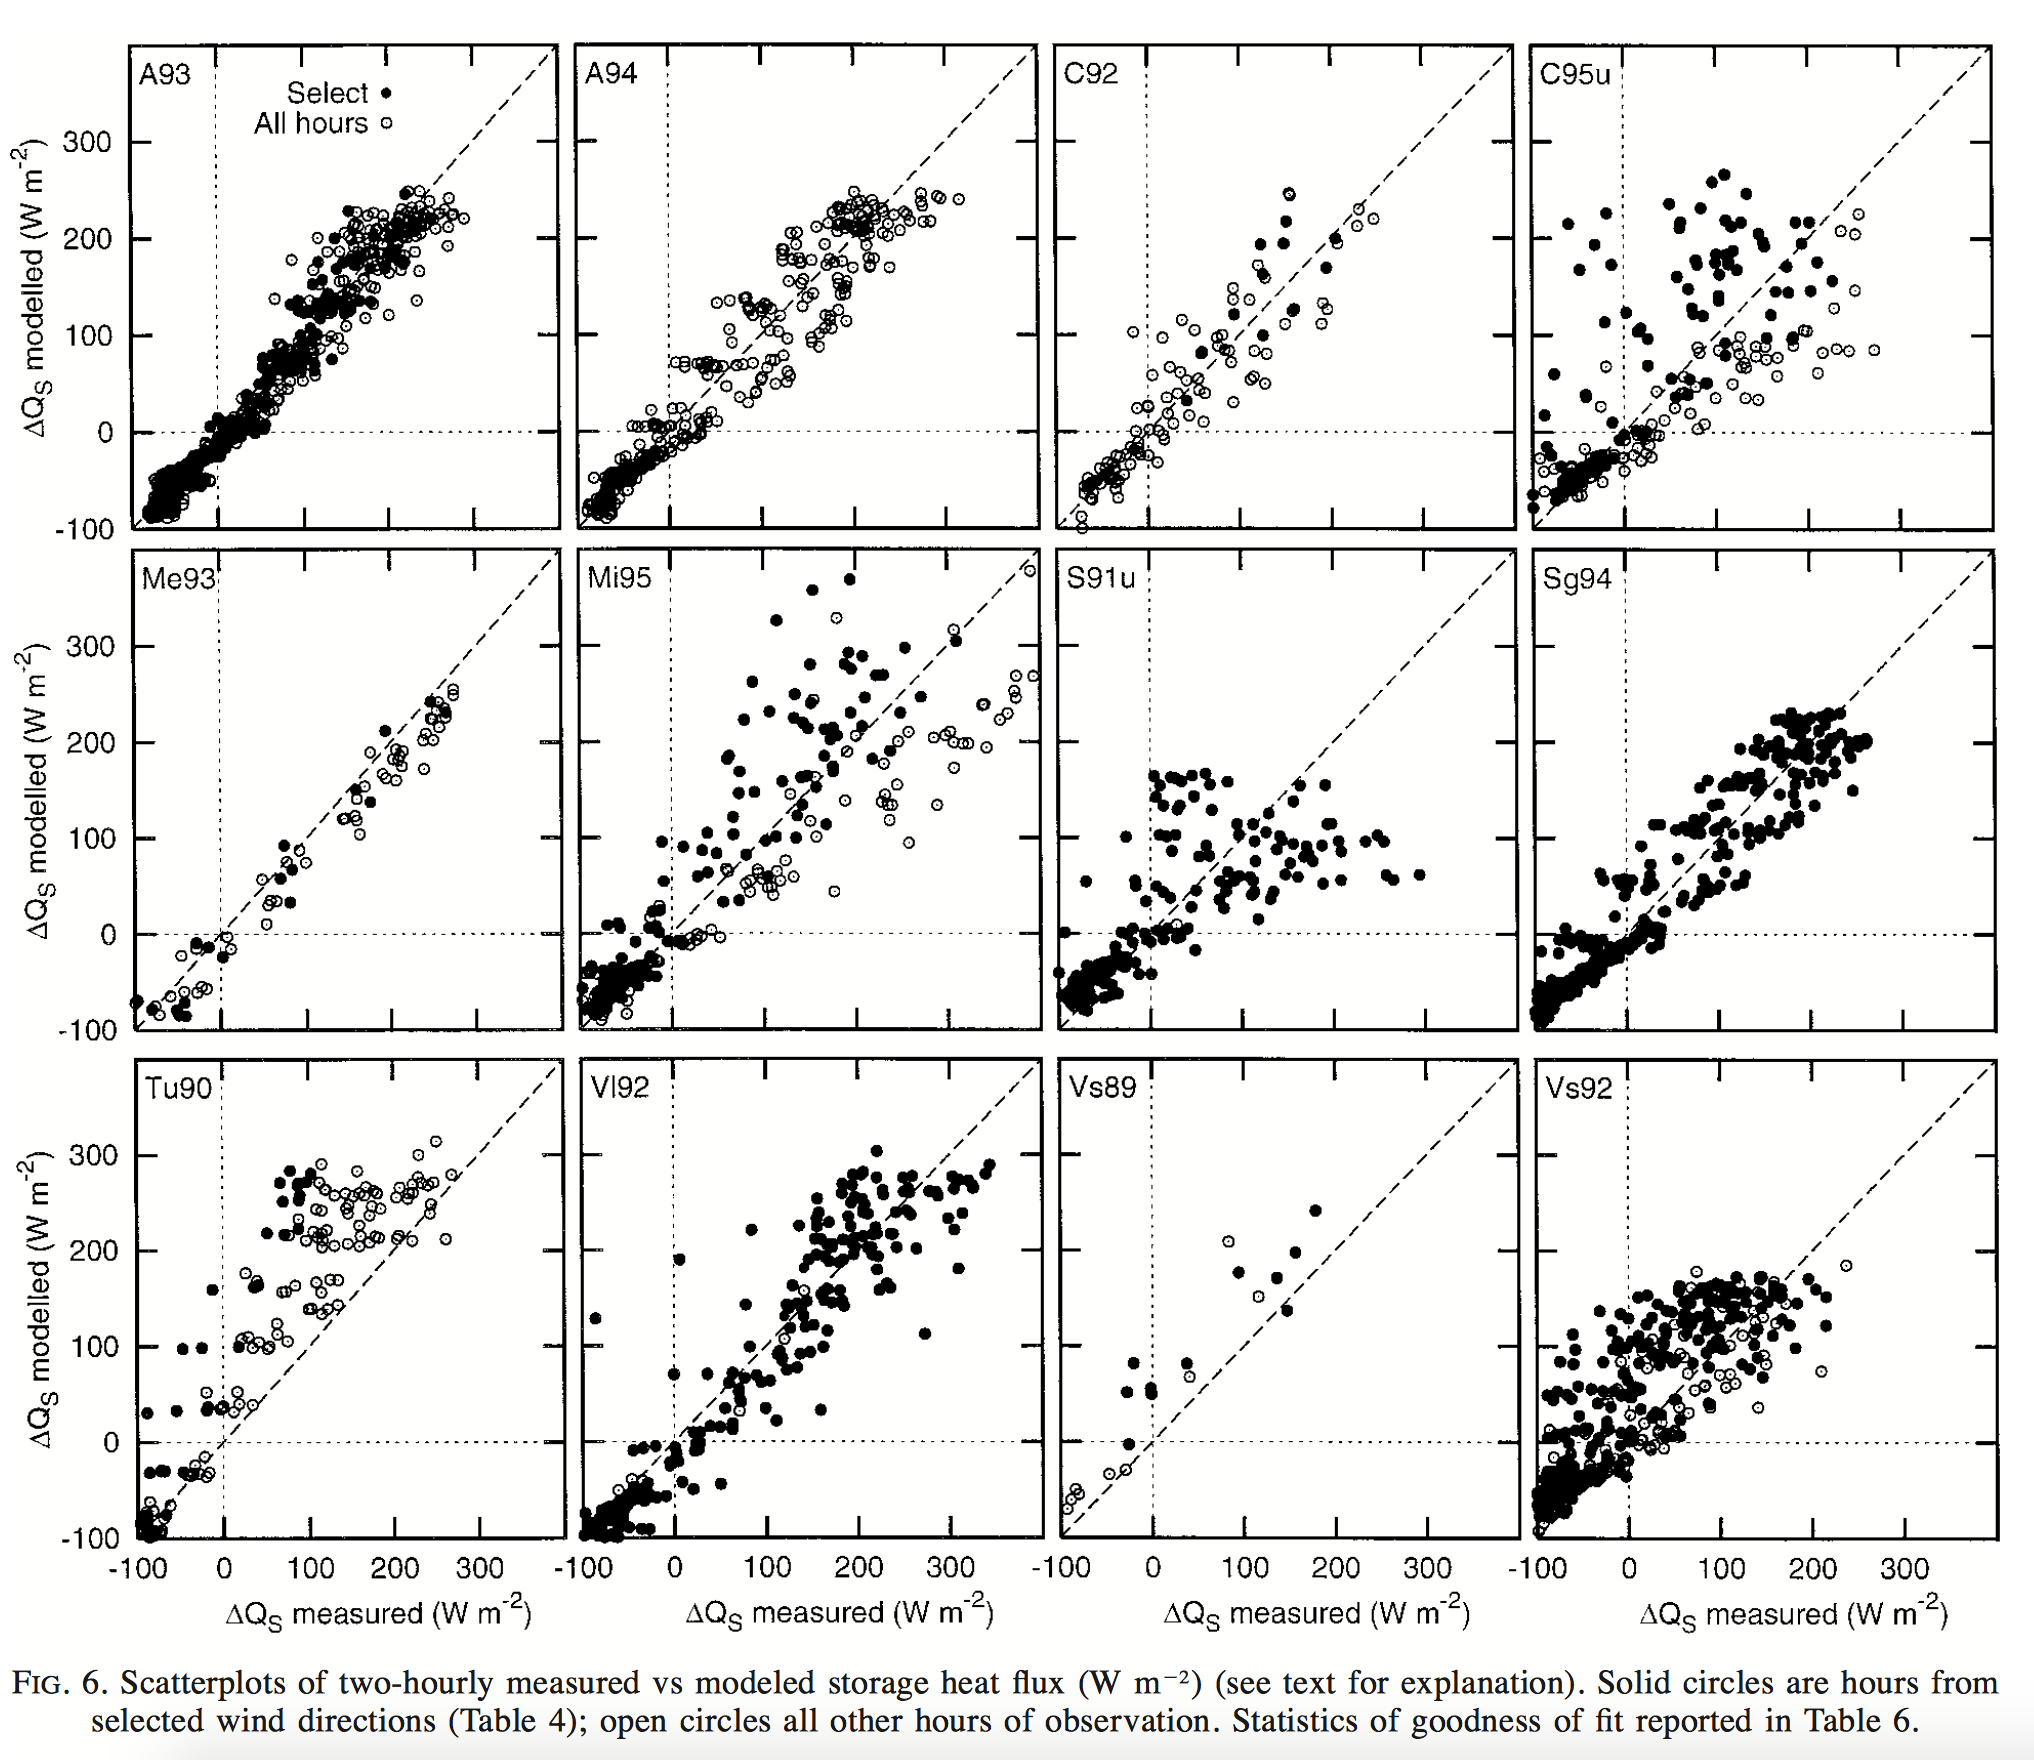
\includegraphics[width=0.8\textwidth]{fig11}
\centering \tiny~\\From Grimmond and Oke (1999) 
\end{figure}
\end{frame}



%------------------------------------------------


\end{document}

